% The manuscript; minimal-winding.pdf beside it is this file built with pdflatex, run three times.
% minimal-winding.typ is a Typst copy of the same text; keep the two in step.
% The figures are figures/minimal-winding.pdf and figures/minimal-winding-paths.pdf, written by ../code/plot_minimal_winding.py.
\documentclass[11pt]{article}
\usepackage[letterpaper,margin=1in]{geometry}
\usepackage[T1]{fontenc}
\usepackage{lmodern}
\usepackage{amsmath,amssymb,amsthm}
\usepackage{graphicx}
\usepackage{array}
\usepackage{microtype}
\usepackage[hidelinks]{hyperref}

\hypersetup{
  pdftitle={Minimal Winding in the Self-Similar Collapse of Three Point Vortices and of Two Concentric Vortex Polygons},
  pdfauthor={Chase Hendrick}}

\newtheorem{theorem}{Theorem}
\newtheorem{lemma}{Lemma}
\newtheorem{proposition}{Proposition}
\newtheorem{corollary}{Corollary}
\theoremstyle{definition}
\newtheorem{remark}{Remark}

\renewcommand{\topfraction}{0.9}
\renewcommand{\textfraction}{0.1}
\renewcommand{\floatpagefraction}{0.8}

\newcommand{\re}{\operatorname{Re}}
\newcommand{\im}{\operatorname{Im}}
\newcommand{\C}{\mathbb{C}}
\newcommand{\Q}{\mathbb{Q}}
\newcommand{\Ap}{\mathcal{A}_+}
\newcommand{\Am}{\mathcal{A}_-}

\title{\Large\bfseries Minimal Winding in the Self-Similar Collapse of\\
  Three Point Vortices and of Two Concentric Vortex Polygons}
\author{Chase Hendrick\\[0.2em] {\small Independent Researcher}\\ {\small\href{mailto:chasewhendrick@gmail.com}{\texttt{chasewhendrick@gmail.com}}}\\ {\small ORCID \href{https://orcid.org/0009-0002-9754-6087}{0009-0002-9754-6087}}}
\date{}

\begin{document}
\maketitle

\begin{abstract}
In a self-similar collapse of point vortices every vortex moves on a logarithmic spiral, and the dimensionless number $P = |\omega_0| t_c$, the initial angular velocity times the collapse time, measures how tightly the spiral winds. We minimize $P$ over two classical collapsing families. Every self-similar collapse of three point vortices can be normalized to circulations $(1, \mu, -\mu/(1 + \mu))$ with $0 < \mu \le 1$ and zero angular impulse. For each $\mu$ the collapsing configurations form two arcs, one for each orientation of the vortex triangle, and $P$ has exactly one critical point, a minimum, on each. The squares of the two minima are roots of an explicit cubic whose coefficients are polynomials in $\mu$, and for $\mu < 1$ the two minima differ. The smaller one increases strictly from $\sqrt{3}/2$, approached as $\mu \to 0$, to $\sqrt{2}$ at $\mu = 1$. Hence $P > \sqrt{3}/2$ for every self-similar collapse of three point vortices, and the constant is sharp; equivalently, every vortex travels more than twice its initial distance from the collision point. For $\mu = 1/2$ the two minima are $1.0647059762\ldots$ and $2.2038550160\ldots$, the positive roots of $8748 \xi^6 - 49005 \xi^4 + 27794 \xi^2 + 18723$, and they are not expressible by real radicals. For two concentric regular $n$-gons with circulations $x_n$ and $-1$, $P = (K_n - \sqrt{2n - 1} \cos n\theta)/(2n \sin n\theta)$ in terms of the relative rotation $\theta$, with an explicit constant $K_n$, and the minimum over $\theta$ is $\sqrt{K_n^2 - 2n + 1}/(2n)$; for pentagons it is $\sqrt{31682}/80$. With a vortex of any circulation added at the center, the minimum over $\theta$ is still explicit and exceeds $\sqrt{3}/2$ for every $n$, and the constant $\sqrt{3}/2$ is again sharp. A strong vortex with weak, tight opposite-signed pairs has $P \ge \sqrt{3}/2 - o(1)$ as the pairs weaken. All formulas are also checked against the Biot--Savart velocities in high-precision arithmetic.

\medskip
\noindent\textbf{Keywords:} point vortices; vortex collapse; self-similar motion; logarithmic spiral.\\
\textbf{MSC 2020:} 76B47, 37N10.
\end{abstract}

\section{Introduction}

Three point vortices collapse self-similarly only if $1/\Gamma_1 + 1/\Gamma_2 + 1/\Gamma_3 = 0$ and their angular impulse about the center of vorticity vanishes (Lemma~\ref{lem:necessary} below). Under these conditions every configuration moves self-similarly: the triangle keeps its shape and rotates while it shrinks to a point in finite time, expands, or rotates rigidly \cite[Sect.~4.5.2]{gallay2026}, \cite{kas2018}. Such collapse was found by Gr\"obli \cite{grobli1877} and found again by Aref \cite{aref1979} and by Novikov and Sedov \cite{ns1979}, who also constructed collapsing configurations of four and five vortices; see \cite[p.~17, Fig.~3]{art1992} for the history and \cite{newton2001} for the general theory. Synge \cite[Sect.~4, Theorem~8]{synge1949} identified $\Gamma_1\Gamma_2 + \Gamma_2\Gamma_3 + \Gamma_3\Gamma_1 = 0$ as an exceptional case: the configurations whose shape lies on a certain conic in his trilinear coordinates then come in one-parameter families of similar triangles, so that the shape does not determine the size. Conte and de Seze \cite{cds1980} solved the motion of three vortices of arbitrary circulations exactly and showed that when $\sum_{j<k} \Gamma_j \Gamma_k = 0$ and the angular impulse vanishes, each vortex runs a logarithmic spiral about the center of vorticity while the triangle keeps its shape, and the configuration either collapses in finite time or expands \cite[Sect.~4]{cds1980}. Kimura \cite{kimura1987} studied similarity solutions of point-vortex systems, Aref \cite{aref2010} derived formulas for the rate of collapse or expansion and the angular frequency of rotation, and Gotoda \cite{gotoda2021} gave explicit formulas for the self-similar motions of three vortices. Borisov and Lebedev \cite{bl1998} obtained conditions for the collapse and the scattering of three vortices within the Lie--Poisson formulation of the problem, and Krishnamurthy, Aref and Stremler \cite{kas2018} recast the motion of three vortices in terms of the circumcircle and the interior angles of the vortex triangle and derived equations of motion for these quantities. Collapse also occurs in configurations of higher symmetry. Aref \cite{aref1982} reduced the motion of two concentric regular $n$-gons of vortices to an integrable Hamiltonian system with two degrees of freedom, and Koiller et al.\ \cite{koiller1985} found collapsing configurations of two such rings, whose vortices move on logarithmic spirals. Demina and Kudryashov \cite[Sect.~3]{dk2014} gave explicitly a family of such configurations that collapse or scatter, with an additional vortex, possibly of zero circulation, at the center, together with the complex constant that determines their rates of collapse and rotation.

In a self-similar collapse at time $t_c$ the configuration has rotated by time $t$ through the angle $-\omega_0 t_c \ln(1 - t/t_c)$, where $\omega_0$ is the initial angular velocity. The angular velocity at time $t$ is $\omega_0 t_c/(t_c - t)$, so the product of the angular velocity and the remaining time does not depend on which instant is taken as initial. Each vortex moves on a logarithmic spiral about the collision point, whose exponent is fixed by this product \cite[p.~298]{ns1979}, \cite[Sect.~4]{cds1980}, \cite[Eq.~(29c)]{aref2010}, \cite[App.~A, Eq.~(A.19)]{dgc2023}, and the dimensionless number $P = |\omega_0| t_c$, which is invariant under rescaling of lengths, times and circulations, is the angle through which the configuration turns while the square of its size decreases by the factor $e$. Equivalently, the path of each vortex makes the constant angle $\arctan 2P$ with the direction to the collision point, and a vortex that starts at distance $r_0$ from that point travels the distance $r_0 \sqrt{1 + 4P^2}$ before the collapse. Kimura \cite{kimura1987} and Aref \cite{aref2010} computed the rate of collapse and the rate of rotation, and the dimensionless combination $P$ of the two rates fixes the spiral \cite[Eq.~(29c)]{aref2010}, but we have not found $P$ minimized in the literature. Within a collapsing family it is natural to ask which configuration winds least.

For three vortices we answer this question for every circulation ratio (Section~\ref{sec:three}). After normalization the circulations are $(1, \mu, -\mu/(1 + \mu))$ with $0 < \mu \le 1$. The collapsing configurations form two arcs, one for each orientation of the triangle, and $P$ has a unique minimum on each (Theorem~\ref{thm:main}). For $\mu < 1$ the two minima differ, and the smaller one increases strictly with $\mu$, from $\sqrt{3}/2$ as $\mu \to 0$ to $\sqrt{2}$ at $\mu = 1$, the value for two equal circulations. Thus $P > \sqrt{3}/2$ for every self-similar collapse of three vortices, and the bound is sharp (Corollary~\ref{cor:bound}); the bound also has a short direct proof from Lemma~\ref{lem:rates} and an elementary inequality. For $\mu = 1/2$ the two minima are conjugate algebraic numbers of degree six, given explicitly in Proposition~\ref{prop:half}. In Section~\ref{sec:rings} we treat two concentric regular $n$-gons, for which the minimization reduces to an elementary inequality once $P$ is written in a suitable form. With a vortex of any circulation at the center the minimum is again explicit; it exceeds $\sqrt{3}/2$ for every $n$ and tends to $\sqrt{3}/2$ as the central circulation grows (Proposition~\ref{prop:centre}). In both families the infimum is approached as a strong vortex carries weak, tight pairs of opposite sign, and Theorem~\ref{thm:pairs} shows that this structure alone forces the constant: for a strong vortex with any number of such pairs, $P \ge \sqrt{3}/2 - o(1)$ as the circulations of the pairs tend to zero, and $P$ comes close to $\sqrt{3}/2$ only if every pair makes the angle $60^\circ$ with the direction away from the strong vortex and all the pairs are at nearly the same distance from it. The theorem is asymptotic; it does not give $P > \sqrt{3}/2$ at a fixed circulation. Section~\ref{sec:numerics} describes an independent numerical check.

\section{Self-similar collapse}

The positions $z_j \in \C$ of point vortices with circulations $\Gamma_j$ evolve according to
\begin{equation}\label{eq:bs}
  \overline{\dot z_j} = \frac{1}{2\pi i} \sum_{k \ne j} \frac{\Gamma_k}{z_j - z_k}.
\end{equation}
Suppose $\sum_j \Gamma_j \ne 0$, let $z_c = \sum_j \Gamma_j z_j / \sum_j \Gamma_j$ be the center of vorticity, which is conserved, and suppose that at $t = 0$ there is $\kappa \in \C$ with $\dot z_j = \kappa (z_j - z_c)$ for all $j$. The right-hand side of \eqref{eq:bs} is homogeneous of degree $-1$ in the relative positions and equivariant under rotations, so the solution is $z_j(t) = z_c + \lambda(t) e^{i\phi(t)} (z_j(0) - z_c)$ with $\lambda \dot\lambda = \re\kappa$ and $\lambda^2 \dot\phi = \im\kappa$. Hence $\lambda^2 = 1 + 2t \re\kappa$. If $\re\kappa < 0$ the vortices collide at $z_c$ at the time $t_c = -1/(2\re\kappa)$, and $\omega_0 = \im\kappa$, so that
\begin{equation}\label{eq:P}
  P = |\omega_0| t_c = \frac{|\im\kappa|}{-2\re\kappa}.
\end{equation}
Integrating $\dot\phi = \omega_0/\lambda^2$ gives $\phi = -P \ln\lambda^2$ when $\omega_0 > 0$, which is the description of the spiral given in the introduction. This is Kimura's similarity solution \cite[Sect.~3.1]{kimura1987}: up to the factor $2\pi$ in his normalization of the circulations, $\kappa$ is his constant $A + iB$, \eqref{eq:P} reads $P = |B|/(-2A)$, and the spirals and the collision time $t_c = -1/(2A)$ are his Eqs.~(3.7) and~(3.9). Earlier, Conte and de Seze \cite[Sect.~4, pp.~24--25]{cds1980} wrote this motion as $z_j = z_{j,0} (1 - t/t_c)^{1/2 - i\omega t_c}$ and gave $-2\omega + i/t_c$ in closed form in their shape variable; there $\omega$ is the initial angular velocity, so $|\omega t_c| = P$. Demina and Kudryashov \cite[Eqs.~(7)--(12)]{dk2014} derive the same solution, like Kimura for any number of vortices but with the normalization of \eqref{eq:bs}, so that their complex constant $c_1$ equals $\kappa$; they give the collapse time $1/(2|\re c_1|)$ \cite[Eq.~(12)]{dk2014} and the rotation angle $(\im c_1/(2\re c_1))\ln(1 + 2t\re c_1)$ \cite[Eq.~(10)]{dk2014}, whose coefficient has absolute value $P$. Gallay and \v{S}ver\'ak \cite[Prop.~5.2, Eqs.~(5.5), (5.11)]{gallay2026} write the collapsing solution as $z_j(t) = (1 - t/T)^{1/2 + is} a_j$ with $z_c = 0$; comparing the two descriptions gives $T = t_c$ and $s = -\omega_0 t_c$, so $|s| = P$. The angular impulse about the center of vorticity satisfies
\begin{equation}\label{eq:L}
  \sum_j \Gamma_j |z_j - z_c|^2 = \frac{1}{\sum_j \Gamma_j} \sum_{j < k} \Gamma_j \Gamma_k |z_j - z_k|^2.
\end{equation}
It is conserved and, in a self-similar motion, proportional to $\lambda^2$, so it must vanish for a collapse. Three of the minimizations below (Remark~\ref{rem:equal} and Propositions~\ref{prop:rings} and~\ref{prop:centre}) and the direct proof of Corollary~\ref{cor:bound} reduce to the following elementary inequality.

\begin{lemma}\label{lem:ineq}
Let $a > |b|$. For $0 < \alpha < \pi$, $(a - b\cos\alpha)/\sin\alpha \ge \sqrt{a^2 - b^2}$, with equality if and only if $\cos\alpha = b/a$.
\end{lemma}

\begin{proof}
The numerator is positive, and $(a - b\cos\alpha)^2 - (a^2 - b^2)\sin^2\alpha = (a\cos\alpha - b)^2$.
\end{proof}

\section{Three vortices}\label{sec:three}

\subsection{Normalization and the collapsing configurations}

The Hamiltonian $H = -(4\pi)^{-1} \sum_{j<k} \Gamma_j \Gamma_k \ln|z_j - z_k|^2$ of \eqref{eq:bs} is conserved. We call a collapse self-similar if all mutual distances are $\lambda(t)$ times their initial values, with $\lambda(t) \to 0$ in finite time.

\begin{lemma}\label{lem:necessary}
In a self-similar collapse of three point vortices all circulations are nonzero, $1/\Gamma_1 + 1/\Gamma_2 + 1/\Gamma_3 = 0$, $\sum_j \Gamma_j \ne 0$, and the angular impulse about the center of vorticity vanishes.
\end{lemma}

\begin{proof}
The harmonic condition and the vanishing of the angular impulse are the classical necessary conditions \cite[Sect.~II~B]{aref2010} (see also \cite[Eqs.~(3.20)--(3.21), (3.33)]{kimura1987}, \cite[Sect.~3]{bl1998} and, for both conditions and any number of vortices, \cite[Eqs.~(26)--(28)]{dk2014}); we include the short argument. Along the motion
\[
  H = H(0) - \frac{1}{4\pi} \Bigl(\sum_{j<k} \Gamma_j \Gamma_k\Bigr) \ln\lambda^2,
\]
and $\ln\lambda^2 \to -\infty$, so $\sum_{j<k} \Gamma_j \Gamma_k = 0$. If one circulation vanished, this would force a second one to vanish; the remaining vortex would then be at rest and the other two would move on circles about it, so no collapse would occur. Hence all $\Gamma_j \ne 0$, and $\sum_{j<k} \Gamma_j \Gamma_k = \Gamma_1\Gamma_2\Gamma_3 \sum_j 1/\Gamma_j$ gives the harmonic condition. Moreover $(\sum_j \Gamma_j)^2 = \sum_j \Gamma_j^2 > 0$. Finally, the angular impulse \eqref{eq:L} is conserved and proportional to $\lambda^2$, so it vanishes.
\end{proof}

By Lemma~\ref{lem:necessary} two of the three circulations of a self-similarly collapsing configuration have the same sign. Multiplying all circulations by a positive constant rescales time and leaves $P$ unchanged. Multiplying them by $-1$ reverses time, and so does complex conjugation of the positions; the composition of the two maps solutions of \eqref{eq:bs} to solutions, and collapsing solutions to collapsing solutions with the same $P$. After relabeling we may therefore assume, as Gotoda does \cite[Sect.~3]{gotoda2021},
\begin{equation}\label{eq:norm}
  \Gamma = \Bigl(1, \mu, -\frac{\mu}{1 + \mu}\Bigr), \quad 0 < \mu \le 1.
\end{equation}
Then $\sum_j \Gamma_j = R/(1 + \mu) > 0$, where $R = 1 + \mu + \mu^2$. For $w = (z_3 - z_1)/(z_2 - z_1)$ the sum $\sum_{j<k} \Gamma_j \Gamma_k |z_j - z_k|^2$ in \eqref{eq:L} equals $\mu(1 + \mu)^{-1} |z_2 - z_1|^2 (1 + 2\mu \re w - (1 + \mu)|w|^2)$, which vanishes exactly on the circle $|w - \mu/(1 + \mu)| = \sqrt{R}/(1 + \mu)$. This circle appears in Kimura \cite[Eqs.~(3.34)--(3.35)]{kimura1987}, who notes that it splits into two arcs of collapse and two of expansion, and in Aref \cite[Eq.~(20a)]{aref2010}; we use the parametrization of it given by Gotoda \cite[Sect.~3]{gotoda2021}:
\begin{equation}\label{eq:pos}
  z_1 = \frac{\mu(1 + \sqrt{R} e^{-i\theta})}{(1 + \mu)^2}, \quad
  z_2 = \frac{\mu - \sqrt{R} e^{-i\theta}}{(1 + \mu)^2}, \quad
  z_3 = 1, \quad \theta \in [0, 2\pi).
\end{equation}
Here $\sum_j \Gamma_j z_j = 0$, so $z_c = 0$, and
\begin{equation}\label{eq:diff}
  z_1 - z_2 = \frac{\sqrt{R} e^{-i\theta}}{1 + \mu}, \quad
  z_3 - z_1 = \frac{\sqrt{R}(\sqrt{R} - \mu e^{-i\theta})}{(1 + \mu)^2}, \quad
  z_3 - z_2 = \frac{\sqrt{R}(\sqrt{R} + e^{-i\theta})}{(1 + \mu)^2}.
\end{equation}
The shape ratio is $w = \mu/(1 + \mu) - (\sqrt{R}/(1 + \mu)) e^{i\theta}$, which traverses the zero-impulse circle exactly once, so every zero-impulse configuration is obtained, up to translation, rotation and dilation, for exactly one $\theta$. Since $\im w = -(\sqrt{R}/(1 + \mu)) \sin\theta$, the triangle $z_1 z_2 z_3$ is negatively oriented for $\sin\theta > 0$ and positively oriented for $\sin\theta < 0$. Put $C = \sqrt{R}\cos\theta$ and
\[
  N(C) = 2(1 + \mu^2) R + (1 - \mu)(2 + \mu + 2\mu^2) C - 2\mu C^2, \quad M(C) = 1 - \mu + 2C.
\]

\begin{lemma}\label{lem:rates}
For every $\theta$ the three quotients $\dot z_j/(z_j - z_c)$ are equal to
\[
  \kappa = \frac{i(1 + \mu)^3}{2\pi\sqrt{R}} \cdot \frac{\sqrt{R} + (1 - \mu) e^{i\theta}}{(\sqrt{R} - \mu e^{i\theta})(\sqrt{R} + e^{i\theta})},
\]
and, with $D = (R + \mu^2 - 2\mu C)(R + 1 + 2C) > 0$,
\[
  \re\kappa = -\frac{(1 + \mu)^3 \mu M(C) \sin\theta}{2\pi\sqrt{R}\, D}, \quad
  \im\kappa = \frac{(1 + \mu)^3 N(C)}{2\pi R D}.
\]
Moreover $N(C) > 0$ for every $\theta$.
\end{lemma}

\begin{proof}
Since $z_c = 0$ and $z_3 = 1$, $\kappa = \dot z_3$, and by \eqref{eq:bs}, $\overline{\dot z_3} = (2\pi i)^{-1} ((z_3 - z_1)^{-1} + \mu (z_3 - z_2)^{-1})$. Inserting \eqref{eq:diff} gives the stated $\kappa$. The same computation for $j = 1$ and $j = 2$ gives the same value, so all three vortices move with the same $\kappa$, in agreement with \cite{kimura1987}, \cite[Sect.~3.1]{ks2018}. The real and imaginary parts follow on multiplying numerator and denominator by the complex conjugate of the denominator, since $|\sqrt{R} - \mu e^{i\theta}|^2 \, |\sqrt{R} + e^{i\theta}|^2 = D$. The two factors of $D$ are at least $(\sqrt{R} - \mu)^2$ and $(\sqrt{R} - 1)^2$, which are positive because $R > \mu^2$ and $R > 1$. Finally, $N$ is concave in $C$, and $N(\sqrt{R}) N(-\sqrt{R}) = 3\mu^2 (1 + \mu)^2 R$ and $N(\sqrt{R}) + N(-\sqrt{R}) = 4R(1 - \mu + \mu^2)$ are positive, so $N > 0$ on $|C| \le \sqrt{R}$.
\end{proof}

Gotoda \cite[Sect.~3]{gotoda2021} gives the rates in this parametrization. In arXiv:2002.09624v1 the imaginary part in his Eq.~(3.3) differs from Lemma~\ref{lem:rates} when $\mu \neq 1$; replacing $(\Gamma_1^2 + \Gamma_2^2)(\Gamma_2\lambda_1 + \Gamma_1\lambda_2)$ there by $(\Gamma_1 + \Gamma_2)(\Gamma_1^2\lambda_1 + \Gamma_2^2\lambda_2)$, in his notation, removes the difference, so we take it to be a misprint.

By Lemma~\ref{lem:rates} every zero-impulse configuration rotates in the positive sense, and it collapses exactly when $M(C) \sin\theta > 0$. Let $\theta_0 \in (0, \pi)$ be defined by $\cos\theta_0 = (\mu - 1)/(2\sqrt{R})$. The configurations with $\theta = 0$ and $\theta = \pi$ are collinear, and those with $\theta = \pm\theta_0$ are equilateral triangles; these four are relative equilibria. The collapsing configurations form the two arcs
\[
  \Ap = (0, \theta_0), \quad \Am = (\pi, 2\pi - \theta_0),
\]
the triangle being negatively oriented on $\Ap$ and positively oriented on $\Am$, and on them \eqref{eq:P} gives
\begin{equation}\label{eq:Ptheta}
  P(\theta) = \frac{N(C)}{2\mu\sqrt{R}\, M(C) \sin\theta}, \quad C = \sqrt{R}\cos\theta.
\end{equation}
Since $z_j(-\theta) = \overline{z_j(\theta)}$, the reflection $\theta \mapsto -\theta$ maps $\Ap$ and $\Am$ onto the expanding arcs $(2\pi - \theta_0, 2\pi)$ and $(\theta_0, \pi)$.

\subsection{The minimal winding}

Let $u = \mu + 1 + 1/\mu \ge 3$ and $Q(\mu, y) = \mu^6 \tilde Q(u, y)$, where
\begin{equation}\label{eq:Q}
\begin{split}
  \tilde Q(u, y) = {}& 1728(u + 1)^2 y^3 - 144(u + 1)(8u^3 - 9u - 9) y^2 \\
  & - 4(16u^6 - 288u^4 - 288u^3 - 81u^2 - 162u - 81) y + 3(4u^3 - 3u - 3)^2.
\end{split}
\end{equation}
Then $Q$ is a polynomial in $\mu$ and $y$ with integer coefficients, irreducible over $\Q$. Its discriminant with respect to $y$ is
\[
  28311552\, \mu^4 (\mu - 1)^2 (\mu + 1)^4 (\mu + 2)^2 (2\mu + 1)^2 R^6 \Delta_1^3,
\]
where $\Delta_1 = 4\mu^6 + 12\mu^5 + 51\mu^4 + 82\mu^3 + 51\mu^2 + 12\mu + 4$; the sum of the roots of $Q(\mu, \cdot)$ is $(8u^3 - 9u - 9)/(12(u + 1)) > 0$, and their product is $-((4u^3 - 3u - 3)/(24(u + 1)))^2 < 0$. Hence for $0 < \mu < 1$ the cubic $Q(\mu, \cdot)$ has three distinct real roots, one negative and two positive, which we denote $y_1(\mu) < y_2(\mu)$.

\begin{theorem}\label{thm:main}
Let $0 < \mu \le 1$.

\textup{(a)} On each of $\Ap$ and $\Am$ the function $P$ has exactly one critical point, and it is the minimum of $P$ on that arc. Denote the two minima by $P_+(\mu)$ and $P_-(\mu)$.

\textup{(b)} $P_+(\mu)^2$ and $P_-(\mu)^2$ are roots of $Q(\mu, \cdot)$. For $\mu < 1$, $P_-(\mu)^2 = y_1(\mu)$ and $P_+(\mu)^2 = y_2(\mu)$, so $P_-(\mu) < P_+(\mu)$; for $\mu = 1$, $P_+ = P_- = \sqrt{2}$.

\textup{(c)} The least value of $P$ over the collapsing configurations, $P_-(\mu)$, is strictly increasing on $(0, 1]$, and $P_-(\mu) \to \sqrt{3}/2$ as $\mu \to 0^+$.
\end{theorem}

\begin{proof}
(a) A direct computation from \eqref{eq:Ptheta} gives
\[
  \frac{dP}{d\theta} = -\frac{G(C)}{2\mu M(C)^2 \sin^2\theta},
\]
where
\begin{equation}\label{eq:K}
  G(C) = 4(1 - \mu) C^3 + 4(2\mu^2 - \mu + 2) C^2 + 2(1 - \mu)^3 C - (2\mu^4 + 7\mu^3 + 6\mu^2 + 7\mu + 2).
\end{equation}
As $\theta$ runs over $\Ap$, $C$ decreases monotonically from $\sqrt{R}$ to $C_0 = (\mu - 1)/2$; over $\Am$ it increases from $-\sqrt{R}$ to $C_0$. The critical points on the two arcs therefore correspond to the roots of $G$ in $(C_0, \sqrt{R})$ and in $(-\sqrt{R}, C_0)$. Now $G(\pm\sqrt{R}) = \pm\sqrt{R}\, N(\pm\sqrt{R}) M(\pm\sqrt{R})/R$, which is positive because $M(\sqrt{R}) > 0 > M(-\sqrt{R})$, and $G(C_0) = -3(1 + \mu)^4/2 < 0$. So $G$ has a root in each interval. For $\mu < 1$, $G$ is a cubic with positive leading coefficient, so it also has a root below $-\sqrt{R}$, and each interval contains exactly one root. For $\mu = 1$, $G = 12C^2 - 24$, with one root in each of $(-\sqrt{3}, 0)$ and $(0, \sqrt{3})$. The function $P$ is differentiable on each arc, and at the ends of each arc $M(C)\sin\theta \to 0$ while $N > 0$, so $P \to +\infty$; hence the single critical point is the minimum.

(b) At a critical point $G(C) = 0$, and since $R\sin^2\theta = R - C^2$, the number $y = P^2$ satisfies $4\mu^2 y (R - C^2) M(C)^2 = N(C)^2$. The resultant of these two polynomials with respect to $C$ is $-48\mu^4 (1 + \mu)^8 Q(\mu, y)$, so $P_\pm(\mu)^2$ are roots of $Q(\mu, \cdot)$ for $\mu < 1$. For $\mu = 1$, $P_\pm = \sqrt{2}$ by Remark~\ref{rem:equal} below, and $Q(1, y) = 6912 (y - 2)^2 (4y + 1)$, so $P_\pm(1)^2 = 2$ is a root of $Q(1, \cdot)$. For $0 < \mu < 1$ both are positive roots, hence each lies in $\{y_1(\mu), y_2(\mu)\}$. The three roots of $G$ are simple, so $P_+(\mu)$ and $P_-(\mu)$ depend continuously on $\mu$, and so do $y_1(\mu) < y_2(\mu)$. By connectedness each of $P_+^2$ and $P_-^2$ coincides with the same $y_i$ on all of $(0, 1)$. At $\mu = 1/2$ the proof of Proposition~\ref{prop:half}, which uses only (a) and the first part of (b), gives certified enclosures $P_-^2 \in [0.99, 1.30]$ and $P_+^2 \in [4.70, 5.02]$, each containing exactly one root of $Q(1/2, \cdot)$; so $P_-^2 = y_1$ and $P_+^2 = y_2$.

(c) For $0 < \mu < 1$ the roots $y_i(\mu)$ are simple, hence differentiable, and $y_i' = -(\partial Q/\partial\mu)/(\partial Q/\partial y)$. A zero of $y_1'$ at some $\mu$ would be a common root of $Q(\mu, \cdot)$ and $(\partial Q/\partial\mu)(\mu, \cdot)$, but their resultant with respect to $y$,
\[
  7044820107264\, \mu^7 (\mu - 1)^3 (\mu + 1)^7 (\mu + 2)^3 (2\mu + 1)^3 R^6 \Delta_2 \Delta_1^3,
\]
where $\Delta_2 = 4\mu^6 + 12\mu^5 + 21\mu^4 + 22\mu^3 + 21\mu^2 + 12\mu + 4$, has no zero in $(0, 1)$. So $y_1$ is strictly monotone on $(0, 1)$. The leading coefficient of $Q(\mu, \cdot)$ does not vanish at $\mu = 1$, so the roots stay bounded as $\mu \to 1^-$, and $y_1$ tends to a nonnegative root of $Q(1, \cdot) = 6912 (y - 2)^2 (4y + 1)$, which is $2$. Since $y_1(1/2) = 1.1335\ldots < 2$, $y_1$ is increasing, and therefore $y_1(\mu) < 2 = P_-(1)^2$ for $\mu < 1$. As $\mu \to 0^+$ it therefore decreases to a limit $L \ge 0$, which is a root of $Q(0, y) = -16(4y - 3)$, so $L = 3/4$. Finally, $y_2 = \sigma - y_1 - y_0 > \sigma - 2$, where $y_0 < 0$ is the negative root and $\sigma = (8u^3 - 9u - 9)/(12(u + 1))$ the sum of the roots; since $\sigma \to \infty$ as $\mu \to 0^+$, $P_+(\mu)$ grows without bound.
\end{proof}

\begin{corollary}\label{cor:bound}
Every self-similar collapse of three point vortices has $|\omega_0| t_c > \sqrt{3}/2$, and for every $\delta > 0$ there is one with $|\omega_0| t_c < \sqrt{3}/2 + \delta$. Equivalently, each vortex travels more than twice its initial distance from the collision point, and the factor $2$ is sharp.
\end{corollary}

\begin{proof}
By Lemma~\ref{lem:necessary}, the normalization \eqref{eq:norm} and Theorem~\ref{thm:main}, $P \ge P_-(\mu) > \sqrt{3}/2$, and $P_-(\mu) \to \sqrt{3}/2$ as $\mu \to 0^+$. The path length is $r_0\sqrt{1 + 4P^2} > 2r_0$, and the angle $\arctan 2P$ between each path and the direction to the collision point exceeds $\arctan\sqrt{3} = \pi/3$; and no vortex starts at the collision point, since $z_1$, $z_2$ and $z_3$ in \eqref{eq:pos} never vanish.
\end{proof}

\begin{proof}[A direct proof of Corollary~\ref{cor:bound}]
The bound needs only Lemmas~\ref{lem:ineq} and~\ref{lem:rates}, not Theorem~\ref{thm:main}. By Lemma~\ref{lem:necessary} and \eqref{eq:norm} it suffices to take $0 < \mu \le 1$ and $\theta \in \Ap \cup \Am$, where $M(C)\sin\theta > 0$. Put $k = (1 - \mu)(2 + \mu)(1 + 2\mu)$, $T = 2R + (1 - \mu)C$ and $V = 3(1 + \mu)^2 (R - C^2) = 3(1 + \mu)^2 R \sin^2\theta > 0$. Comparing coefficients of $\mu$ in the first identity and of $C$ in the other two shows
\[
  k^2 + 27\mu^2(1 + \mu)^2 = 4R^3, \qquad
  T^2 = R M(C)^2 + V, \qquad
  9(1 + \mu)^2 N(C) = 2R(T^2 + V) + k M(C) T;
\]
in the third, the coefficients of $C^2$, $C$ and $1$ on each side are $-18\mu(1 + \mu)^2$, $9(1 - \mu)(1 + \mu)^2(2 + \mu + 2\mu^2)$ and $18(1 + \mu)^2(1 + \mu^2)R$. By the first identity there is $\psi \in (0, \pi)$ with $\cos\psi = k/(2R^{3/2})$ and $\sin\psi = 3\sqrt{3}\,\mu(1 + \mu)/(2R^{3/2})$. By the second, $T \ne 0$, and $x = \sqrt{R}\,M(C)/T$ and $y = \sqrt{V}/|T|$ satisfy $x^2 + y^2 = 1$ and $0 < |x| < 1$. The third, divided by $2RT^2$, reads $9(1 + \mu)^2 N(C)/(2RT^2) = 2 - x^2 + x\cos\psi$, and $2|x|y\sin\psi = 9\mu(1 + \mu)^2 M(C)\sin\theta/(\sqrt{R}\,T^2)$, so \eqref{eq:Ptheta} becomes
\[
  P = \frac{2 - x^2 + x\cos\psi}{2|x|\,y\sin\psi}.
\]
Lemma~\ref{lem:ineq} with $a = 2 - x^2$ and $b = -x$, where $a - |b| = (1 - |x|)(2 + |x|) > 0$, gives $2|x|yP \ge \sqrt{(2 - x^2)^2 - x^2}$, and $(2 - x^2)^2 - x^2 = 3x^2y^2 + 4y^4$ because $x^2 + y^2 = 1$. Hence
\[
  P^2 \ge \frac34 + \frac{y^2}{x^2} = \frac34 + \frac{3(1 + \mu)^2 \sin^2\theta}{M(C)^2} > \frac34 .
\]
Equivalently, with $N = N(C)$ and $M = M(C)$, the three identities combine into
\[
  4R^3\bigl(N^2 - 3\mu^2(R - C^2)M^2\bigr) = (kN + 3\mu^2 MT)^2 + 48\mu^2(1 + \mu)^2R^2(R - C^2)^2 .
\]
For sharpness, take $\theta$ with $\sin\theta = -\sqrt{3}\,\mu/2$ and $C = -\sqrt{R}\sqrt{1 - 3\mu^2/4}$, which lies in $\Am$ because $C < -1/2 \le (\mu - 1)/2 = \sqrt{R}\cos\theta_0$. As $\mu \to 0$, $C + \sqrt{R} = 3\mu^2/8 + O(\mu^3)$; by the proof of Lemma~\ref{lem:rates}, $N(-\sqrt{R}) = 3\mu^2(1 + \mu)^2R/N(\sqrt{R}) = 3\mu^2/4 + O(\mu^3)$; and $N'(C) = 2 + O(\mu)$ near $C = -1$. So $N(C) = 3\mu^2/2 + O(\mu^3)$, $M(C) = -1 + O(\mu)$, and \eqref{eq:Ptheta} gives $P = \sqrt{3}/2 + O(\mu)$. The remaining statements follow as in the first proof.
\end{proof}

Every motion of three point vortices in the plane that ends in a total collision is self-similar \cite[Theorem~1]{hgl2007}, \cite[Prop.~2.8]{hiraoka2008}, \cite[Sect.~3]{hiraoka2009}, \cite[Sect.~3.1]{ks2018}, \cite[Prop.~5.2]{gallay2026}, \cite[Theorem~1.1]{drivas2026}, so the bound of Corollary~\ref{cor:bound} holds for every collapse of three point vortices. The bound fails for more vortices: the collapsing configuration of seven vortices in \cite[Table~1, Fig.~1a]{dk2014}, with circulation $6383/2250$ at the origin, $14/15$ at $\pm 2$, $-62/45$ at $\pm 2e^{i\varphi}$ where $\cos 2\varphi = 13/18$, and $1$ at $\pm 4/3$, has the constant $\Omega = 12433/9000 - (31\sqrt{155}/450)\,i$, where $\Omega = 2\pi i\,\overline{\kappa}$ \cite[Eq.~(11)]{dk2014}, so $P = |\re\Omega|/(2|\im\Omega|) = 12433/(1240\sqrt{155}) = 0.8053\ldots < \sqrt{3}/2$.

\begin{figure}[t]
  \centering
  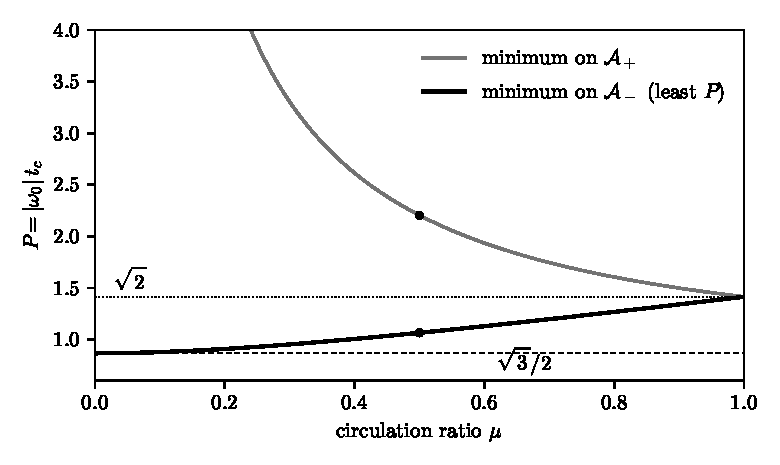
\includegraphics[width=0.78\textwidth]{figures/minimal-winding.pdf}
  \caption{The minima $P_-(\mu)$ and $P_+(\mu)$ of $P = |\omega_0| t_c$ on the two collapsing arcs, as functions of the circulation ratio $\mu$. The dots mark $\mu = 1/2$ (Proposition~\ref{prop:half}). As $\mu \to 0$, $P_-$ tends to $\sqrt{3}/2$ and $P_+$ grows without bound.}
  \label{fig:minima}
\end{figure}

The two minima are shown in Figure~\ref{fig:minima}, and Figure~\ref{fig:paths} shows two minimizing configurations and the paths of their vortices.

\begin{figure}[t]
  \centering
  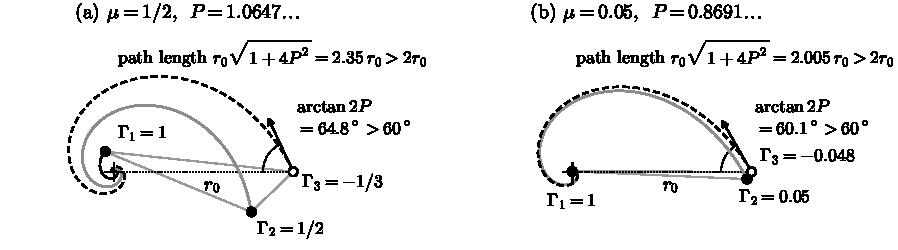
\includegraphics[width=0.95\textwidth]{figures/minimal-winding-paths.pdf}
  \caption{Minimizing configurations on $\Am$ (dots, filled for positive circulation) and the logarithmic spiral paths of their vortices into the collision point ($+$), drawn until the distances have shrunk by the factor $100$, for (a) $\mu = 1/2$ and (b) $\mu = 0.05$, where the two weak vortices form a tight pair beside the strong one, as in Theorem~\ref{thm:pairs}, and $P$ is close to $\sqrt{3}/2$. Each path meets the line to the collision point at the constant angle $\arctan 2P > 60^\circ$ and has length $r_0\sqrt{1 + 4P^2} > 2r_0$ (Corollary~\ref{cor:bound}), marked here for the third vortex.}
  \label{fig:paths}
\end{figure}

\subsection{The ratio \texorpdfstring{$\mu = 1/2$}{mu = 1/2}}

For $\Gamma = (1, 1/2, -1/3)$ we have $R = 7/4$ and $\cos\theta_0 = -\sqrt{7}/14$, and \eqref{eq:Ptheta} becomes
\[
  P(\theta) = \frac{14\sin^2\theta + 6\sqrt{7}\cos\theta + 21}{2(14\cos\theta + \sqrt{7})\sin\theta}.
\]

\begin{proposition}\label{prop:half}
Let $X = 245351/5201^{3/2}$ and $\sigma = 7\sqrt{5201}/162$. For $\mu = 1/2$,
\[
  P_- = \sqrt{\frac{605}{324} + \sigma\cos\Bigl(\frac13 \arccos X - \frac{2\pi}{3}\Bigr)} = 1.0647059762712043\ldots,
\]
\[
  P_+ = \sqrt{\frac{605}{324} + \sigma\cos\Bigl(\frac13 \arccos X\Bigr)} = 2.2038550160361327\ldots,
\]
attained at $\cos\theta = -0.9243893679\ldots$ and $\cos\theta = 0.6739838839\ldots$ respectively. Both are roots of the polynomial $8748\xi^6 - 49005\xi^4 + 27794\xi^2 + 18723$, which is irreducible over $\Q$ and whose real roots are exactly these two numbers and their negatives.
\end{proposition}

\begin{proof}
Here $16\,Q(1/2, \xi^2) = 8748\xi^6 - 49005\xi^4 + 27794\xi^2 + 18723$, and by Theorem~\ref{thm:main}(b) the squares of both minima are roots of this polynomial. As a cubic in $q = \xi^2$ it is irreducible over $\Q$ and has positive discriminant, so its roots are real and are given by the trigonometric solution of the cubic, $q_m = 605/324 + \sigma\cos(\frac13 \arccos X - 2\pi m/3)$, $m = 0, 1, 2$, with $q_0 \approx 4.856977$, $q_1 \approx 1.133599$ and $q_2 \approx -0.388724$. The critical points are the roots of $G$ in the two intervals of the proof of Theorem~\ref{thm:main}(a); with $C = (\sqrt{7}/2)\cos\theta$ they are at the stated values of $\cos\theta$. Exact sign changes of $G$ place them in $0.67 < \cos\theta < 0.68$ on $\Ap$ and $-0.93 < \cos\theta < -0.92$ on $\Am$, and interval arithmetic applied to $P^2 = N^2/(4\mu^2 (R - C^2) M^2)$ on these intervals gives $P_+^2 \in [4.70, 5.02]$ and $P_-^2 \in [0.99, 1.30]$. Each enclosure contains exactly one of $q_0, q_1, q_2$, so $P_+^2 = q_0$ and $P_-^2 = q_1$.
\end{proof}

\begin{remark}\label{rem:radicals}
The two minima are conjugate algebraic numbers of degree six. Since the cubic in $q$ is irreducible over $\Q$ and has three real roots, none of its roots is expressible by real radicals (casus irreducibilis), and therefore neither minimum is. The same holds for every $\mu = a/b \in (0, 1)$ in lowest terms with $2 \le b \le 30$: for each of these 277 values, $Q(\mu, \xi^2)$ is irreducible over $\Q$, so the minima have degree six and the cubic $Q(\mu, \cdot)$ is irreducible, and its discriminant is positive on $(0, 1)$, so it has three real roots.
\end{remark}

\begin{remark}\label{rem:equal}
For $\mu = 1$, that is $\Gamma = (1, 1, -1/2)$, the zero-impulse circle is $|w - 1/2| = \sqrt{3}/2$. With $w = 1/2 + (\sqrt{3}/2) e^{i\beta}$, $z_1 = 0$ and $z_2 = 1$, the same computation gives $P = (3 - \cos 2\beta)/(2\sin 2\beta)$ on the collapsing arcs $0 < \beta < \pi/2$ and $\pi < \beta < 3\pi/2$, which are exchanged by interchanging the two equal vortices ($w \mapsto 1 - w$). Since $P$ has period $\pi$ in $\beta$, Lemma~\ref{lem:ineq} applies on both arcs and gives $P \ge \sqrt{2}$, with equality if and only if $\cos 2\beta = 1/3$, in agreement with Theorem~\ref{thm:main}. This parametrization is Kimura's \cite[Sect.~4]{kimura1987}, who gives the two rates for $\Gamma = (2, 2, -1)$ in his Eq.~(4.4); their ratio $B/(-2A)$ is this expression for $P$, which is also a specialization and reparametrization of Gr\"obli's spiral coefficient \cite[Sect.~10]{grobli1877}.
\end{remark}

\begin{remark}\label{rem:swap}
Interchanging the first two vortices and multiplying the circulations by $1/\mu$ maps the family with ratio $\mu$ onto the family with ratio $1/\mu$ and exchanges the two orientations, so the arc minima satisfy $P_+(\mu) = P_-(1/\mu)$. For $\mu > 1$ the smaller minimum is therefore attained on $\Ap$.
\end{remark}

\section{Two concentric regular polygons}\label{sec:rings}

In this section $\theta$ denotes the relative rotation of two rings. Let $n \ge 2$ and $\epsilon = e^{2\pi i/n}$, and place vortices of circulation $x > 0$ at $z\epsilon^k$ and vortices of circulation $-1$ at $\zeta\epsilon^k$, $k = 0, \dots, n - 1$. The motion preserves this symmetry, and the center of vorticity is the origin. Using
\[
  \sum_{k=1}^{n-1} \frac{1}{1 - \epsilon^k} = \frac{n - 1}{2}, \quad
  \sum_{k=0}^{n-1} \frac{1}{z - \zeta\epsilon^k} = \frac{n z^{n-1}}{z^n - \zeta^n},
\]
one finds that \eqref{eq:bs} reduces to \cite[Eq.~(3)]{aref1982}
\begin{equation}\label{eq:rings}
  \overline{\dot z} = \frac{1}{2\pi i}\Bigl(\frac{x(n - 1)}{2z} - \frac{n z^{n-1}}{z^n - \zeta^n}\Bigr), \quad
  \overline{\dot\zeta} = \frac{1}{2\pi i}\Bigl(-\frac{n - 1}{2\zeta} + \frac{x n \zeta^{n-1}}{\zeta^n - z^n}\Bigr).
\end{equation}
A collapse requires the angular impulse $n(x|z|^2 - |\zeta|^2)$ to vanish, and after a rotation and a dilation we take $z = 1$ and $\zeta = \sqrt{x}\, e^{i\theta}$. The motion is self-similar exactly when $\dot z/z = \dot\zeta/\zeta$. Writing $v = \zeta^n$, \eqref{eq:rings} gives
\[
  \overline{\dot z/z} = \frac{1}{2\pi i}\Bigl(\frac{x(n - 1)}{2} - \frac{n}{1 - v}\Bigr), \quad
  \overline{\dot\zeta/\zeta} = \frac{1}{2\pi i}\Bigl(-\frac{n - 1}{2x} - \frac{n v}{1 - v}\Bigr),
\]
and these are equal if and only if
\begin{equation}\label{eq:circ}
  (n - 1)x^2 - 2nx + (n - 1) = 0.
\end{equation}
This is the circulation condition of Koiller et al.\ \cite[Sect.~11]{koiller1985}. Demina and Kudryashov \cite[Sect.~3]{dk2014} place circulations $\Gamma_1$ and $\Gamma_2 = -\Gamma_1/r^2$ on two such rings, where $r$ is the ratio of the radii, and a vortex of circulation $\Gamma_0$ at the center; for $\Gamma_0 = 0$ their equation for $r$ \cite[Eq.~(37)]{dk2014} is \eqref{eq:circ} with $x = r^2$. The condition \eqref{eq:circ} coincides with the classical condition $\sum_{i<j} \Gamma_i \Gamma_j = 0$ for the $2n$ vortices, whose left side here equals $(n/2)((n - 1)x^2 - 2nx + (n - 1))$. Its roots are $x_n$ and $1/x_n$, where
\[
  x_n = \frac{n + \sqrt{2n - 1}}{n - 1} = e^\eta, \quad \cosh\eta = \frac{n}{n - 1}.
\]
The root $1/x_n$ gives the same family with the two rings interchanged, as one sees by multiplying the circulations by $-x_n$ and reflecting the configuration, so we take $x = x_n$. Then every $\theta$ gives a self-similar motion. Let $\rho = x_n^{n/2} = e^{n\eta/2} > 1$ and $\alpha = n\theta$, so that $v = \rho e^{i\alpha}$. The common value of $\overline{\kappa}$ is $S/(2\pi i)$ with $S = x_n(n - 1)/2 - n/(1 - v)$, so $\kappa = (\im S + i\re S)/(2\pi)$, and since $\im(1 - v)^{-1} = \rho\sin\alpha/|1 - v|^2$,
\[
  \re\kappa = -\frac{n\rho\sin\alpha}{2\pi|1 - v|^2}.
\]
The configuration therefore collapses exactly when $\sin n\theta > 0$, that is, for $0 < \theta < \pi/n$ modulo $2\pi/n$. Using $|1 - v|^2 = 1 - 2\rho\cos\alpha + \rho^2$ one finds
\[
  \frac{|1 - v|^2 \re S}{\rho} = K_n - ((n - 1)x_n - n)\cos\alpha, \quad
  K_n = \frac{(n - 1)x_n(\rho + \rho^{-1})}{2} - \frac{n}{\rho}.
\]
Here $(n - 1)x_n - n = \sqrt{2n - 1}$, and writing $n = (n - 1)\cosh\eta$ in the last term of $K_n$ gives
\[
  K_n = (n - 1)\sinh\frac{(n + 2)\eta}{2}.
\]
Moreover
\[
  K_n - \sqrt{2n - 1} = \frac{(n - 1)x_n(\rho^{1/2} - \rho^{-1/2})^2}{2} + n(1 - \rho^{-1}) > 0,
\]
so $\re S > 0$, and \eqref{eq:P} gives
\begin{equation}\label{eq:Pring}
  P = \frac{K_n - \sqrt{2n - 1}\cos n\theta}{2n\sin n\theta}, \quad 0 < n\theta < \pi.
\end{equation}
The collapse rate and the rotation rate as functions of the relative angle are given by Koiller et al.\ \cite[Sect.~11]{koiller1985}. The constant $S$ is the constant $\Omega$ of \cite[Eq.~(11)]{dk2014}, and Demina and Kudryashov write it for these rings, with the central vortex, as an explicit function of $e^{in\theta}$ \cite[Eq.~(36)]{dk2014}; for $\Gamma_0 = 0$, $\Gamma_1 = x_n$ and radii $1$ and $\sqrt{x_n}$ their expression reduces to $S$ by \eqref{eq:circ}. Equation~\eqref{eq:Pring} writes the ratio of the two rates in closed form.

\begin{proposition}\label{prop:rings}
For $n \ge 2$ the collapsing configurations of two concentric regular $n$-gons with circulations $x_n$ and $-1$ satisfy
\[
  P \ge F_n = \frac{\sqrt{K_n^2 - (2n - 1)}}{2n},
\]
with equality if and only if $\cos n\theta = \sqrt{2n - 1}/K_n$.
\end{proposition}

\begin{proof}
Apply Lemma~\ref{lem:ineq} to \eqref{eq:Pring} with $a = K_n$ and $b = \sqrt{2n - 1}$.
\end{proof}

For small $n$ the constants are as follows.
\begin{center}
\renewcommand{\arraystretch}{1.35}
\begin{tabular}{|c|c|c|c|c|}
  \hline
  $n$ & $x_n$ & $K_n$ & $F_n$ & $\cos n\theta$ at the minimum \\ \hline
  $2$ & $2 + \sqrt{3}$ & $4\sqrt{3}$ & $3\sqrt{5}/4$ & $1/4$ \\ \hline
  $3$ & $(3 + \sqrt{5})/2$ & $11$ & $\sqrt{29}/3$ & $\sqrt{5}/11$ \\ \hline
  $4$ & $(4 + \sqrt{7})/3$ & $55\sqrt{7}/9$ & $\sqrt{322}/9$ & $9/55$ \\ \hline
  $5$ & $2$ & $127\sqrt{2}/8$ & $\sqrt{31682}/80$ & $12\sqrt{2}/127$ \\ \hline
\end{tabular}
\end{center}
For $n = 2$ the configuration is a parallelogram of four vortices; Novikov and Sedov \cite[Sect.~4]{ns1979} found this collapse and its rates, so its minimum $F_2$ follows from their formulas, and Gotoda \cite{gotoda2021} gives its rates in closed form. The ratio $x_n$ is rational exactly when $2n - 1$ is a perfect square, and $n = 5$ is the smallest such $n$. There $x_5 = 2$ and
\[
  P = \frac{127\sqrt{2} - 24\cos 5\theta}{80\sin 5\theta} \ge \frac{\sqrt{31682}}{80} = 2.2249297741726591\ldots.
\]

Now place a vortex of circulation $\Gamma_0$ at the center as well. The velocity that each ring induces at the center vanishes, so this vortex stays at rest, and it does not change the angular impulse. It adds $\Gamma_0$ to the bracket in the expression for $\overline{\dot z/z}$ above and $\Gamma_0/x$ to the bracket for $\overline{\dot\zeta/\zeta}$, so the two quotients are equal if and only if
\begin{equation}\label{eq:circ0}
  (n - 1)x^2 - 2(n - \Gamma_0)x + (n - 1) - 2\Gamma_0 = 0, \quad\text{that is,}\quad \Gamma_0 = \frac{(n - 1)x^2 - 2nx + n - 1}{2(1 - x)},
\end{equation}
and again every $\theta$ gives a self-similar motion. On \eqref{eq:circ0} the total circulation does not vanish, since $2(x - 1)(n(x - 1) + \Gamma_0) = (n + 1)x^2 - 2nx + n + 1 > 0$, so the center of vorticity is the origin. The left side of \eqref{eq:circ0} equals $-2$ at $x = 1$ and $n - 1 - 2\Gamma_0$ at $x = 0$, so for every real $\Gamma_0$ it has exactly one root $x > 1$, and for $\Gamma_0 < (n - 1)/2$ also exactly one root in $(0, 1)$. Multiplying the circulations by $-1/x$ and reflecting the configuration, as for $\Gamma_0 = 0$, interchanges the rings and maps the root $x < 1$ for $\Gamma_0$ to the root $1/x > 1$ for $-\Gamma_0/x$, with the same $P$. So we take $x > 1$ and write $x = e^{2t}$ with $t > 0$. With $A = x(n - 1)/2 + \Gamma_0$, the common value of $\overline{\kappa}$ is $S/(2\pi i)$ with $S = A - n/(1 - v)$.

\begin{proposition}\label{prop:centre}
Let $n \ge 2$ and $\Gamma_0 \in \mathbb{R}$, and let $x = e^{2t}$, $t > 0$, be the root of \eqref{eq:circ0} greater than $1$. The configuration with relative rotation $\theta$ collapses exactly when $\sin n\theta > 0$, and then
\begin{equation}\label{eq:Pcentre}
  P = \frac{a - b\cos n\theta}{2n\sin n\theta}, \quad a = \coth t\cosh nt + n\sinh nt, \quad b = \coth t .
\end{equation}
Hence $P \ge \sqrt{D^2 - n^2}/(2n)$, where $D = \coth t\sinh nt + n\cosh nt > 2n$, with equality if and only if $\cos n\theta = b/a$. This minimum over $\theta$ exceeds $\sqrt{3}/2$ and decreases strictly from $\infty$ to $\sqrt{3}/2$ as $\Gamma_0$ increases from $-\infty$ to $\infty$; with $h = 1/(\Gamma_0 - 1/2)$ it is
\[
  \frac{\sqrt{3}}{2} + \frac{\sqrt{3}\,(1 + 2n^2)}{36}\,h^2 + O(h^4) \quad \text{as } \Gamma_0 \to +\infty.
\]
In particular $P > \sqrt{3}/2$ for every $n \ge 2$, every $\Gamma_0$ and both roots of \eqref{eq:circ0}, and no larger constant holds for all of them.
\end{proposition}

\begin{proof}
The central vortex does not change $\im S = -n\rho\sin\alpha/|1 - v|^2$, so the configuration collapses exactly when $\sin n\theta > 0$, and the computation that led to \eqref{eq:Pring} gives $|1 - v|^2 \re S/\rho = a - b\cos\alpha$ with $a = A(\rho + \rho^{-1}) - n/\rho$ and $b = 2A - n$. By \eqref{eq:circ0}, $A = (n + 1)/2 + 1/(x - 1) = (n + \coth t)/2$, and with $\rho = e^{nt}$ this gives the stated $a$ and $b$. Since $a \mp b = \coth t\,(\cosh nt \mp 1) + n\sinh nt > 0$, $\re S > 0$, and \eqref{eq:P} gives \eqref{eq:Pcentre}. Lemma~\ref{lem:ineq} gives the minimum $\sqrt{a^2 - b^2}/(2n)$, and $a^2 - b^2 = D^2 - n^2$ because $\cosh^2 nt - \sinh^2 nt = 1$. The difference $\sinh nt - n\sinh t$ vanishes at $t = 0$ and has derivative $n(\cosh nt - \cosh t) \ge 0$, so $\coth t\sinh nt \ge n\cosh t > n$; with $n\cosh nt > n$ this gives $D > 2n$, and hence $D^2 - n^2 > 3n^2$. Moreover $\coth t\sinh nt = \cosh t\sum_{j=0}^{n-1} e^{(n - 1 - 2j)t}$, where the sum pairs into terms $2\cosh((n - 1 - 2j)t)$, plus $1$ when $n$ is odd, so $D$ increases strictly with $t$, from $2n$ as $t \to 0$ to $\infty$. By \eqref{eq:circ0}, $\Gamma_0 = (n + \coth t)/2 - (n - 1)e^{2t}/2$, which decreases strictly from $\infty$ to $-\infty$ as $t$ increases; this gives the monotonicity and the two limits. Finally, $D$ is even in $t$, with $D = 2n + n(1 + 2n^2)t^2/3 + O(t^4)$, and $\Gamma_0 - 1/2 = 1/(2t) + O(t)$, so $h = 2t + O(t^3)$ and $(D^2 - n^2)/(4n^2) = 3/4 + (1 + 2n^2)h^2/12 + O(h^4)$, which gives the expansion. The root $x < 1$ reduces to a root $x > 1$ by the interchange of the rings described above.
\end{proof}

For $\Gamma_0 = 0$ the root greater than $1$ is $x_n = e^\eta$, so $t = \eta/2$. Since $n = (n - 1)\cosh\eta$ and $(n - 1)\sinh\eta = \sqrt{2n - 1}$, we get $b = \coth(\eta/2) = \sqrt{2n - 1}$ and $a = (n - 1)\sinh((n + 2)\eta/2) = K_n$, so \eqref{eq:Pcentre} is \eqref{eq:Pring} and the minimum is $F_n$ of Proposition~\ref{prop:rings}; in particular $F_n > \sqrt{3}/2$ for every $n$. The family and its rates are those of Demina and Kudryashov \cite[Sect.~3, Eqs.~(36)--(37)]{dk2014}: their Eq.~(37) with $\Gamma_1 = r^2 = x$ is $x$ times \eqref{eq:circ0}, and on \eqref{eq:circ0} their constant $\Omega$ is $S$. For $n = 2$ the configuration is the five-vortex collapse of Novikov and Sedov \cite{ns1979}, a parallelogram with a vortex where its diagonals cross, and Gotoda gives its rates in closed form \cite{gotoda2021}, in his Eq.~(3.13) in arXiv:2002.09624v1. These sources give the rates, but none of them minimizes or bounds their ratio. Proposition~\ref{prop:centre} does not conflict with the seven-vortex collapse with $P = 0.8053\ldots$ in Section~\ref{sec:three}, which has three concentric 2-gons around the central vortex, not two.

In Corollary~\ref{cor:bound} the value $\sqrt{3}/2$ is approached as $\mu \to 0$, and in Proposition~\ref{prop:centre} as $\Gamma_0 \to +\infty$; in both limits a strong vortex carries weak, tight pairs of opposite sign. For three vortices this picture appears in Krishnamurthy and Stremler \cite[Sect.~3.6, Fig.~9]{ks2018}: as their parameter $g$ tends to $-1$ they describe a small vortex dipole moving in the field of a strong, fixed vortex, and on their slice $A = \pi/3$ the self-induced motion of the dipole makes the angle $\pi/3$ with the motion induced by the strong vortex; they compute collapse times and the energy, not the rotation or $P$. We show that this structure alone forces the constant $\sqrt{3}/2$, for any number of pairs.

Let $m \ge 1$ and $0 < c \le 1$. We consider $1 + 2m$ point vortices: one of circulation $1$ at the origin and, for $j = 1, \dots, m$, one of circulation $\gamma a_j$ at $Z_j$ and one of circulation $-\gamma b_j$ at $W_j$, where $\gamma > 0$ and, for all $j$ and all $l \ne j$,
\begin{equation}\label{eq:class}
  c \le a_j, b_j \le \frac{1}{c}, \quad c \le |Z_j| \le \frac{1}{c}, \quad c\gamma|Z_j| \le |W_j - Z_j| \le \frac{\gamma|Z_j|}{c}, \quad |Z_j - Z_l| \ge c.
\end{equation}
We write $d_j = W_j - Z_j$ and
\[
  u_j = \frac{d_j}{\gamma a_j Z_j} = p_j + iy_j, \qquad \nu_j = \frac{a_j - b_j}{\gamma a_j^2},
\]
so that $W_j = Z_j(1 + \gamma a_j u_j)$, $b_j = a_j(1 - \gamma a_j\nu_j)$ and, by \eqref{eq:class}, $c^2 \le |u_j| \le c^{-2}$. Pair $j$ has length $\gamma a_j|u_j||Z_j|$, and $\arg u_j$ is the angle from the direction $Z_j$, away from the strong vortex, to the direction from the positive to the negative vortex of the pair. The normalization is no loss of generality: a translation puts the strong vortex at the origin, multiplying all circulations by a positive constant leaves $P$ unchanged, and the map $(\Gamma_i, z_i) \mapsto (-\Gamma_i, \overline{z_i})$ of Section~\ref{sec:three} sends $\kappa$ to $\overline{\kappa}$ and keeps $P$, so a strong vortex of negative circulation is covered as well.

\begin{theorem}[A strong vortex with weak tight pairs]\label{thm:pairs}
Let $m \ge 1$ and $0 < c \le 1$, and consider configurations as above that collapse self-similarly, that is, $\dot z_i = \kappa(z_i - z_c)$ for all $1 + 2m$ vortices, with $\re\kappa < 0$.

\textup{(a)} For every $\delta > 0$ there is $\gamma_1 > 0$, depending only on $m$, $c$ and $\delta$, such that every such collapse with $\gamma < \gamma_1$ has $P > \sqrt{3}/2 - \delta$.

\textup{(b)} For every $\delta > 0$ there are $\eta > 0$ and $\gamma_2 > 0$, depending only on $m$, $c$ and $\delta$, such that every such collapse with $\gamma < \gamma_2$ and $P < \sqrt{3}/2 + \eta$ has $|u_j - e^{i\pi/3}| < \delta$, $|\nu_j - 1| < \delta$ and $\bigl||Z_j|/|Z_l| - 1\bigr| < \delta$ for all $j$ and $l$.

\textup{(c)} For every $\delta > 0$ and $\bar P > 0$ there is $\gamma_3 > 0$, depending only on $m$, $c$, $\delta$ and $\bar P$, such that every such collapse with $\gamma < \gamma_3$ and $P \le \bar P$ has, for every $j$, $|p_j - 1/2| < \delta$, $|\nu_j - 1| < \delta$, $y_j > 0$ and
\[
  \Bigl|P - \frac{y_j^2 + 3/4}{2y_j}\Bigr| < \delta, \qquad \text{where} \quad \frac{y_j^2 + 3/4}{2y_j} = \frac{\sqrt{3}}{2} + \frac{(y_j - \sqrt{3}/2)^2}{2y_j}.
\]
For every $m$, the constant $\sqrt{3}/2$ in \textup{(a)} cannot be increased when $c$ is small enough.
\end{theorem}

So, for weak pairs, $P$ is close to $\sqrt{3}/2$ only if every pair has length close to $\gamma a_j|Z_j|$ and makes the angle $60^\circ$ with the direction away from the strong vortex, all the pairs are at nearly the same distance from the strong vortex, and the negative circulation of each pair, $-\gamma a_j + \gamma^2 a_j^2\nu_j$, agrees up to $o(\gamma^2)$ with the three-vortex harmonic value $-\gamma a_j/(1 + \gamma a_j)$.

\begin{proof}
It suffices to prove three statements about a sequence of such collapses with $\gamma = \gamma_n \to 0$, in which we write $P_n$, $\kappa_n$, $u_{j,n} = p_{j,n} + iy_{j,n}$, and so on:
(S1) $\liminf P_n \ge \sqrt{3}/2$;
(S2) if $P_n \to \sqrt{3}/2$, then $u_{j,n} \to e^{i\pi/3}$, $\nu_{j,n} \to 1$ and $|Z_{j,n}|/|Z_{l,n}| \to 1$ for all $j$ and $l$;
(S3) if $\sup_n P_n < \infty$, then for every $j$, $p_{j,n} \to 1/2$, $\nu_{j,n} \to 1$, $\liminf_n y_{j,n} > 0$ and $P_n - (y_{j,n}^2 + 3/4)/(2y_{j,n}) \to 0$.
Indeed, if (a) failed for some $\delta$, there would be a sequence with $\gamma_n \to 0$ and $P_n \le \sqrt{3}/2 - \delta$, contrary to (S1). If (b) failed for some $\delta$, there would be a sequence with $\gamma_n \to 0$ and $P_n < \sqrt{3}/2 + 1/n$ for which one of the inequalities fails for every $n$, and after passing to a subsequence it is always the same inequality, for the same $j$ and $l$; by (S1), $P_n \to \sqrt{3}/2$, contrary to (S2). The same argument with $P_n \le \bar P$ reduces (c) to (S3).

Throughout, $\gamma \le \gamma_0 = c^3/(8m)$, and $O(\gamma^k)$ denotes a quantity bounded by $\gamma^k$ times a constant that depends only on $m$ and $c$. Each identity used below is a direct computation, verified in \texttt{verify\_strong\_vortex.py} (Section~\ref{sec:numerics}).

\emph{Step 1: a priori bounds.} By \eqref{eq:class}, $|d_j| \le \gamma/c^2 \le c/8$. Hence $|W_j| \ge c/2$; every vortex of pair $j$ is at distance at least $c - 2\gamma/c^2 \ge c/2$ from every vortex of pair $l \ne j$; and $\sum_i \Gamma_i = 1 + \gamma\sum_j (a_j - b_j)$ lies in $[1/2, 2]$. The identity
\begin{equation}\label{eq:zc}
  \sum_i \Gamma_i z_i = \sum_j \bigl(\gamma(a_j - b_j)Z_j - \gamma b_j d_j\bigr)
\end{equation}
gives $|\sum_i \Gamma_i z_i| \le 2m\gamma/c^2$, so that $|z_c| \le 4m\gamma/c^2 \le c/2$ and $|Z_j - z_c| \ge c/2$. The contribution of pair $l$ to the sum in \eqref{eq:bs} at a point $z$ is
\[
  f_l(z) = \frac{\gamma a_l}{z - Z_l} - \frac{\gamma b_l}{z - W_l} = \frac{\gamma(a_l - b_l)}{z - Z_l} - \frac{\gamma b_l d_l}{(z - Z_l)(z - W_l)}.
\]
At the vortices of a pair $j \ne l$ it satisfies $|f_l| \le 4\gamma/c^2$, and
\[
  f_l(W_j) - f_l(Z_j) = d_j\Bigl(\frac{\gamma b_l}{(W_j - W_l)(Z_j - W_l)} - \frac{\gamma a_l}{(W_j - Z_l)(Z_j - Z_l)}\Bigr)
\]
gives $|f_l(W_j) - f_l(Z_j)| \le 8\gamma|d_j|/c^3$. Finally, $|\gamma b_j/d_j| \le c^{-3}$.

\emph{Step 2: the equations of a pair.} With the strong vortex at the origin, the equation $\dot z_i = \kappa(z_i - z_c)$ at $Z_j$, and the difference of the equations at $W_j$ and $Z_j$, in which $z_c$ cancels, read by \eqref{eq:bs}
\begin{align}
  2\pi i\,\overline{\kappa}\,\overline{(Z_j - z_c)} &= \frac{1}{Z_j} + \frac{\gamma b_j}{d_j} + \sum_{l \ne j} f_l(Z_j), \label{eq:pairZ}\\
  2\pi i\,\overline{\kappa}\,\overline{d_j} &= -\frac{d_j}{Z_jW_j} + \frac{\gamma(a_j - b_j)}{d_j} + \sum_{l \ne j} \bigl(f_l(W_j) - f_l(Z_j)\bigr). \label{eq:pairD}
\end{align}
By Step~1 the right side of \eqref{eq:pairZ} has absolute value at most $1/c + 1/c^3 + 4m\gamma/c^2 \le 3/c^3$, and $|Z_j - z_c| \ge c/2$, so $|\kappa| \le 3/(\pi c^4)$.

\emph{Step 3: the relative motion.} Multiply \eqref{eq:pairD} by $Z_j/(\gamma a_j)$ and write $-d_j/(Z_jW_j) = -d_j/Z_j^2 + d_j^2/(Z_j^2W_j)$. Since $d_j = \gamma a_j u_j Z_j$, the multiplication turns $\overline{d_j}$ into $|Z_j|^2\,\overline{u_j}$, $\gamma(a_j - b_j)/d_j$ into $\nu_j/u_j$, $-d_j/Z_j^2$ into $-u_j$, and $d_j^2/(Z_j^2W_j)$ into $\gamma a_j u_j^2/(1 + \gamma a_j u_j)$. Hence, by Step~1,
\begin{equation}\label{eq:rel}
  2\pi i\,\overline{\kappa}\,|Z_j|^2\,\overline{u_j} = -u_j + \frac{\nu_j}{u_j} + \rho_j, \qquad |\rho_j| \le \gamma\Bigl(\frac{2}{c^5} + \frac{8(m - 1)}{c^7}\Bigr) \le \frac{1}{c^4}.
\end{equation}
Since $|\kappa|$, $|Z_j|$, $|u_j|$ and $1/|u_j|$ are bounded, \eqref{eq:rel} bounds $\nu_j$, for instance $|\nu_j| \le 8c^{-10}$; this uses no information on $b_j/a_j$. So $a_j - b_j = \gamma a_j^2 \nu_j = O(\gamma)$: the total circulation of each pair is $O(\gamma^2)$. Three consequences follow. By \eqref{eq:zc}, $\sum_i \Gamma_i z_i = \sum_j (\gamma^2 a_j^2 \nu_j Z_j - \gamma b_j d_j) = O(\gamma^2)$, so $z_c = O(\gamma^2)$. Next, $b_j/a_j = 1 - \gamma a_j\nu_j = 1 + O(\gamma)$. And by the second form of $f_l$, $f_l(Z_j) = O(\gamma^2)$ for $l \ne j$, although the bound $O(\gamma)$ of Step~1 suffices below. Multiplying \eqref{eq:pairZ} by $Z_j$ and using $\gamma b_j Z_j/d_j = (b_j/a_j)/u_j$ and $\overline{(Z_j - z_c)}\,Z_j = |Z_j|^2 - \overline{z_c}\,Z_j$, we obtain
\begin{equation}\label{eq:rate}
  2\pi i\,\overline{\kappa}\,|Z_j|^2 = 1 + \frac{1}{u_j} + O(\gamma).
\end{equation}

\emph{Step 4: the angular impulse.} The angular impulse about $z_c$ vanishes (Section~2). With the strong vortex at the origin, $\sum_i \Gamma_i |z_i - z_c|^2 = \sum_i \Gamma_i |z_i|^2 - |z_c|^2 \sum_i \Gamma_i$, and pair $j$ contributes
\[
  \gamma a_j|Z_j|^2 - \gamma b_j|W_j|^2 = \gamma^2|Z_j|^2\bigl(a_j^2\nu_j - 2a_jb_jp_j - \gamma a_j^2 b_j|u_j|^2\bigr)
\]
to $\sum_i \Gamma_i|z_i|^2$. Since $z_c = O(\gamma^2)$ and $a_jb_j = a_j^2 - \gamma a_j^3\nu_j$, dividing by $\gamma^2$ gives
\begin{equation}\label{eq:imp}
  \sum_j a_j^2|Z_j|^2(\nu_j - 2p_j) = O(\gamma).
\end{equation}
Here $z_c = O(\gamma^2)$ is needed: the a priori bound $z_c = O(\gamma)$ would leave a term of order $1$.

\emph{Step 5: limits.} Along the sequence, $a_j$, $Z_j$, $u_j$, $\nu_j$ and $\kappa$ are bounded, so every subsequence has a further subsequence along which they converge, to $a_j^*$, $Z_j^*$, $u_j^* = p_j^* + iy_j^*$, $\nu_j^*$ and $\kappa^*$. Then $b_j \to a_j^*$, $a_j^* \ge c$, $|Z_j^*| \ge c$, $|u_j^*| \ge c^2$ and $\re\kappa^* \le 0$, and \eqref{eq:rate}, \eqref{eq:rel} and \eqref{eq:imp} become
\begin{equation}\label{eq:limit}
  2\pi i\,\overline{\kappa^*}\,|Z_j^*|^2 = 1 + \frac{1}{u_j^*}, \quad
  2\pi i\,\overline{\kappa^*}\,|Z_j^*|^2\,\overline{u_j^*} = -u_j^* + \frac{\nu_j^*}{u_j^*}, \quad
  \sum_j a_j^{*2}|Z_j^*|^2(\nu_j^* - 2p_j^*) = 0.
\end{equation}
Eliminating $\kappa^*$ between the first two and multiplying by $u_j^*$ gives
\[
  2p_j^{*2} + p_j^* - \nu_j^* + iy_j^*(2p_j^* - 1) = 0,
\]
so $y_j^*(2p_j^* - 1) = 0$ and $\nu_j^* = 2p_j^{*2} + p_j^*$. By the first equation, $\kappa^* = i\,\overline{(1 + 1/u_j^*)}/(2\pi|Z_j^*|^2)$, that is,
\begin{equation}\label{eq:kstar}
  \re\kappa^* = -\frac{y_j^*}{2\pi|Z_j^*|^2|u_j^*|^2}, \qquad \im\kappa^* = \frac{1 + p_j^*/|u_j^*|^2}{2\pi|Z_j^*|^2}
\end{equation}
for every $j$.

\emph{Case A: some $y_j^* \ne 0$.} Then $\im(1 + 1/u_j^*) = -y_j^*/|u_j^*|^2 \ne 0$, so $2\pi i\,\overline{\kappa^*}$ is not real, and the first equation of \eqref{eq:limit} shows $y_l^* \ne 0$ for every $l$. Hence $p_l^* = 1/2$ and $\nu_l^* = 1$ for every $l$, and since $\re\kappa^* \le 0$, \eqref{eq:kstar} gives $y_l^* > 0$ for every $l$ and $\re\kappa^* < 0$. So $P$, a continuous function of $\kappa$ on $\re\kappa < 0$, converges along the subsequence to
\[
  P^* = \frac{\im\kappa^*}{-2\re\kappa^*} = \frac{|u_l^*|^2 + p_l^*}{2y_l^*} = \frac{y_l^{*2} + 3/4}{2y_l^*} = \frac{\sqrt{3}}{2} + \frac{(y_l^* - \sqrt{3}/2)^2}{2y_l^*} \ge \frac{\sqrt{3}}{2},
\]
the same number for every $l$. Thus every $y_l^*$ is one of the two positive roots, $y^*$ and $3/(4y^*)$, of $y^2 - 2P^*y + 3/4$; different pairs may take different roots, and they then lie at different distances from the strong vortex, by the first equation of \eqref{eq:limit}. If $P^* = \sqrt{3}/2$, the two roots coincide, every $y_l^* = \sqrt{3}/2$, so $u_l^* = e^{i\pi/3}$, and the first equation of \eqref{eq:limit} gives the same $|Z_l^*|$ for every $l$.

\emph{Case B: every $y_j^* = 0$.} Then $1 + 1/u_j^*$ is real, so $\kappa^*$ is purely imaginary. If $\kappa^* \ne 0$, then $\re\kappa_n \to 0^-$ while $|\im\kappa_n| \to |\kappa^*| > 0$, so $P_n \to \infty$ along the subsequence. If $\kappa^* = 0$, then $1 + 1/p_j^* = 0$, so $p_j^* = -1$ and $\nu_j^* = 1$ for every $j$, and the last equation of \eqref{eq:limit} reads $3\sum_j a_j^{*2}|Z_j^*|^2 = 0$, which is impossible. This is the only place where the angular impulse enters.

\emph{Conclusion.} Every subsequence has a further subsequence along which either $P_n \to \infty$, or Case~A holds and $P_n \to P^* \ge \sqrt{3}/2$; this proves (S1). If $P_n \to \sqrt{3}/2$, only Case~A with $P^* = \sqrt{3}/2$ can occur, so every subsequence has a further subsequence along which $u_{j,n} \to e^{i\pi/3}$, $\nu_{j,n} \to 1$ and $|Z_{j,n}|/|Z_{l,n}| \to 1$; since these limits do not depend on the subsequence, the whole sequence converges to them, which proves (S2). If $\sup_n P_n < \infty$, only Case~A can occur, and the same argument gives $p_{j,n} \to 1/2$, $\nu_{j,n} \to 1$ and $P_n - (y_{j,n}^2 + 3/4)/(2y_{j,n}) \to 0$, while $\liminf_n y_{j,n} > 0$ because every subsequence has a further subsequence along which $y_{j,n}$ has a positive limit; this proves (S3). Finally, the families of Corollary~\ref{cor:bound} and Proposition~\ref{prop:centre} contain collapses that satisfy \eqref{eq:class}, for $m = 1$ and for every $m = n \ge 2$, and have $P \to \sqrt{3}/2$, as shown next; so $\sqrt{3}/2$ in (a) cannot be increased.
\end{proof}

The two families lie in the class \eqref{eq:class} near their minima. For three vortices, translate vortex~$1$ to the origin and take $m = 1$, $\gamma = \mu$, $a_1 = 1$, $b_1 = 1/(1 + \mu)$, $Z_1 = z_2 - z_1$ and $W_1 = z_3 - z_1$ in \eqref{eq:pos}; then $\nu_1 = 1/(1 + \mu)$ and $|Z_1| = \sqrt{R}/(1 + \mu)$, and along the configurations with $\sin\theta = -\sqrt{3}\,\mu/2$ used for sharpness in the direct proof of Corollary~\ref{cor:bound}, $u_1 \to e^{i\pi/3}$ as $\mu \to 0$. For the rings of Proposition~\ref{prop:centre} with $\Gamma_0 > 0$, divide the circulations by $\Gamma_0$ and take $m = n$, $\gamma = 1/\Gamma_0$, $a_j = x$, $b_j = 1$, $Z_j = \epsilon^j$ and $W_j = \sqrt{x}\,e^{i\theta}\epsilon^j$; then $\nu_j = (x - 1)\Gamma_0/x^2 \to 1$ as $\Gamma_0 \to +\infty$, and at the minimizing $\theta$, where $\cos n\theta = b/a$ in \eqref{eq:Pcentre}, $\theta/t \to \sqrt{3}$ and $u_j = (\sqrt{x}\,e^{i\theta} - 1)\Gamma_0/x \to e^{i\pi/3}$. In both cases \eqref{eq:class} holds for all small $\gamma$, with $c = 1/2$ for three vortices and $c = \min(1/2, 2\sin(\pi/n))$ for the rings, and $P \to \sqrt{3}/2$ by Corollary~\ref{cor:bound} and Proposition~\ref{prop:centre}. This is why the same constant appears in both results. Theorem~\ref{thm:pairs} does not reprove them: it is asymptotic and gives no bound at a fixed $\gamma > 0$, and for three vortices the fact that a bounded $P$ forces a tight pair as $\mu \to 0$ comes from the exact formulas of Section~\ref{sec:three}, not from the theorem. Nor does it say anything about collapses outside its hypotheses, and these cannot simply be dropped: the seven-vortex collapse of Section~\ref{sec:three}, with $P = 0.8053\ldots < \sqrt{3}/2$, has no dominant vortex, since its other circulations are $0.33$, $0.35$ and $0.49$ times the central one, and the nearest vortices of opposite sign in it are separated by $0.38$ times their distance from the center.

\section{Numerical verification}\label{sec:numerics}

The results were checked numerically as summarized in Table~\ref{tab:checks}. Except where the table says otherwise, the checks evaluate the Biot--Savart velocities \eqref{eq:bs} directly for configurations built independently of \eqref{eq:pos} (two vortices fixed and the third moved around the zero-impulse circle), test self-similarity by comparing $\dot z_j/(z_j - z_c)$ across all vortices, and obtain $P$ from \eqref{eq:P}. The algebraic steps in the proofs were verified in exact arithmetic (SymPy): Lemma~\ref{lem:rates} for all three vortices, \eqref{eq:K}, the resultant in the proof of Theorem~\ref{thm:main}(b), the discriminant and the resultant in the proof of Theorem~\ref{thm:main}(c), the irreducibility of $Q$ and of each of the 277 sextics in Remark~\ref{rem:radicals}, the constants in Proposition~\ref{prop:half}, and, for general $n$, the identities of Section~\ref{sec:rings} from \eqref{eq:circ} to \eqref{eq:Pring}, together with the table of constants. The program \texttt{verify\_general\_mu.py} carries out these exact computations with SymPy~1.14.0 and the high-precision checks with mpmath~1.3.0; \texttt{verify\_floors\_independent.py} repeats the minimizations independently and contains the exact sign changes of $G$ and the interval enclosures in the proof of Proposition~\ref{prop:half}, computed with the interval arithmetic of mpmath at 30 digits. The program \texttt{verify\_direct\_proof.py} checks every identity in the direct proof of Corollary~\ref{cor:bound} exactly, with SymPy. The program \texttt{verify\_central\_vortex.py} checks Proposition~\ref{prop:centre}: exactly, with SymPy, the derivation of \eqref{eq:circ0} and \eqref{eq:Pcentre} for symbolic $n$, every identity in the proof, the case $\Gamma_0 = 0$ and the expansion, and also the leading-order relations used in Step~5 of the proof of Theorem~\ref{thm:pairs}, with the limits of $u_j$ and $P$ along the two families; numerically, the Biot--Savart velocities and the minima over $\theta$ at 50 and 30 digits; and negative controls, checks that must fail and do. The program \texttt{verify\_strong\_vortex.py} checks Theorem~\ref{thm:pairs}: exactly, with SymPy, every identity its proof uses; numerically, exact self-similar solutions for $1 + 2m$ vortices with $m = 1$ and $m = 3$ at $\gamma = 10^{-2}$, $10^{-3}$ and $10^{-4}$, checked by direct Biot--Savart, along which $P$ stays above $\sqrt{3}/2$ and approaches it; and negative controls. Its output is \texttt{data/verify-strong-vortex-2026-09-25.txt}. Each program runs in under a minute under Python~3.11 and prints every check with its result; their output is in \texttt{data/}.

\begin{table}[tp]
  \centering
  \small
  \renewcommand{\arraystretch}{1.2}
  \begin{tabular}{|>{\raggedright\arraybackslash}p{0.555\textwidth}|>{\raggedright\arraybackslash}p{0.39\textwidth}|}
    \hline
    \textbf{Check} & \textbf{Result} \\ \hline
    Lemma~\ref{lem:rates} against the Biot--Savart velocities of all three vortices, at the positions \eqref{eq:pos} for 36 pairs $(\mu, \theta)$ on a grid with $0.1 \le \mu \le 7$, and for 30 triangles built independently of \eqref{eq:pos}, 50 digits
      & relative difference $\le 2 \times 10^{-49}$ \\ \hline
    Arc minima by direct minimization of $P$, computed from the quotient of the first vortex, for 26 values of $\mu \in (0, 1]$ at 30 digits and 13 rational values at 50 digits
      & agree with the roots of $Q(\mu, \cdot)$ to $5 \times 10^{-21}$ and $5 \times 10^{-45}$ \\ \hline
    $\mu = 1/2$: the three quotients over 4000 shapes on the zero-impulse circle, 60 digits
      & equal to 60-digit working precision; the collapsing shapes fill half of the circle, the arcs $\mathcal{A}_\pm$ \\ \hline
    $\mu = 1/2$: local minima of $P$ over the collapsing shapes, located numerically
      & two, equal to the values of Proposition~\ref{prop:half} to 60-digit working precision \\ \hline
    $\mu = 1/2$: formula for $P(\theta)$ against direct evaluation at the positions \eqref{eq:pos}, 399 interior points of each arc
      & relative difference $\le 10^{-59}$ \\ \hline
    $\mu = 1/2$: integration of \eqref{eq:bs} from the minimizing configuration on $\Am$ (Taylor method, 30 digits)
      & every $|z_j - z_c|^2$ follows $1 - t/t_c$, and every rotation angle follows $-\omega_0 t_c \ln(1 - t/t_c)$, to 30-digit working precision up to $t = 0.9\, t_c$ \\ \hline
    Five configurations at the positions \eqref{eq:pos} with $\mu \in \{0.3, 0.5, 2\}$, on both arcs: integration of \eqref{eq:bs} to $t = 0.9\, t_c$ (fourth-order Runge--Kutta, 30 digits)
      & distances to the collision point, rotation angles, the angle $\arctan 2P$ between each velocity and the direction to the collision point, and path lengths $r_0 \sqrt{1 + 4P^2}\,(1 - \sqrt{1 - t/t_c})$ agree to $2 \times 10^{-10}$ \\ \hline
    $\mu = 1$ (Remark~\ref{rem:equal}): $P$ from \eqref{eq:bs} against $(3 - \cos 2\beta)/(2\sin 2\beta)$ on both collapsing arcs, and its minimum, 50 digits
      & difference $\le 2 \times 10^{-47}$; minimum $\sqrt{2}$ at $\cos 2\beta = 1/3$ on both arcs \\ \hline
    $\mu = 1$: the configuration with the fastest collapse at $|z_1 - z_2| = 1$, 50 digits
      & $\cos 2\beta = 3/5$, $t_c = 4\pi/3$ and $P = 3/2$ to $10^{-40}$ \\ \hline
    $\mu = 1$: Kimura's rates $A$, $B$ \cite[Eq.~(4.4)]{kimura1987} at ten angles in $0 < \beta < \pi/2$, 50 digits
      & $\kappa = (A + iB)/(4\pi)$ for $\Gamma = (1, 1, -1/2)$, to $10^{-45}$ \\ \hline
    Two rings, $n = 2, \dots, 10$: the reduced equations \eqref{eq:rings} and the two sums over roots of unity against the full Biot--Savart sum, 50 digits
      & difference $\le 10^{-49}$ \\ \hline
    Two rings, $n = 2, \dots, 8$: $P$ from \eqref{eq:bs} against \eqref{eq:Pring} over the collapsing range, and its numerical minimum against $F_n$, 60 digits
      & relative difference $\le 3 \times 10^{-58}$; minima agree to $2 \times 10^{-60}$ \\ \hline
    Two rings: the equations of Demina and Kudryashov \cite[Eqs.~(36)--(37)]{dk2014} at $\Gamma_0 = 0$ (exact, SymPy), and their constant against the Biot--Savart sum, $n = 2, \dots, 8$, 50 digits
      & (37) is \eqref{eq:circ} with $x = r^2$; (36) minus $S$ is a multiple of \eqref{eq:circ}; difference $\le 10^{-45}$ \\ \hline
    The collapsing configuration of seven vortices in \cite[Table~1, Fig.~1a]{dk2014}, Biot--Savart at 50 digits
      & self-similar, the printed $\Omega$ to $10^{-45}$, and $P = 12433/(1240\sqrt{155}) < \sqrt{3}/2$ \\ \hline
    Two rings with a central vortex, $n \in \{2, 3, 4, 5, 7\}$, $-1999.5 \le \Gamma_0 \le 250$, each positive root of \eqref{eq:circ0}: Biot--Savart for all $2n + 1$ vortices, 295 configurations, 50 digits; minima over $\theta$, 13 cases, 30 digits
      & quotients equal to $\kappa$ to $3 \times 10^{-48}$, $P$ to \eqref{eq:Pcentre} to $6 \times 10^{-41}$, \cite[Eq.~(36)]{dk2014} holds to $3 \times 10^{-48}$; minima $\sqrt{D^2 - n^2}/(2n)$ to $4 \times 10^{-27}$ \\ \hline
    Theorem~\ref{thm:pairs}: exact self-similar solutions, $m = 1$ and $m = 3$ weak pairs, $\gamma = 10^{-2}, 10^{-3}, 10^{-4}$, direct Biot--Savart
      & $P$ stays above $\sqrt{3}/2$ and approaches it \\ \hline
  \end{tabular}
  \caption{Numerical checks of the results.}
  \label{tab:checks}
\end{table}

\section{Discussion}

Lemma~\ref{lem:rates} gives, in a form suited to minimization, the collapse and rotation rates that Aref \cite[Eqs.~(25a), (25d)]{aref2010} expresses through the side lengths of the triangle (see also \cite{gotoda2021}, \cite[Eq.~(E.1)]{gallay2026}, and, for equal circulations, \cite[Eq.~(4.4)]{kimura1987}); Aref also notes that the rotation rate times the collapse time, that is, the ratio of the two rates, fixes the logarithmic spiral \cite[Eq.~(29c)]{aref2010}. Theorem~\ref{thm:main} concerns the minimization of that ratio, which neither \cite{aref2010}, \cite{cds1980} nor \cite{kimura1987} considers. When the two circulations of the same sign differ, $\mu < 1$, the two orientations of the triangle are not equivalent and the minima on the two arcs differ, so a minimization restricted to one orientation finds only one of them. The infimum $\sqrt{3}/2$ of Corollary~\ref{cor:bound} is approached only as $\mu \to 0$ and is not attained.

Leoncini, Kuznetsov and Zaslavsky \cite{lkz2000} analyze the motion near collapse when two of the vortices are identical; the configuration that collapses fastest at a fixed distance between the identical vortices, found by Kimura \cite[Eq.~(4.6)]{kimura1987} and shown in \cite[Fig.~18]{lkz2000}, has $P = 3/2$, and the value $\sqrt{3}/2$ in that caption is a value of their energy parameter $\Lambda = e^{4\pi H}$, not of $P$. For $\sum_{j<k} \Gamma_j \Gamma_k = 0$, Tavantzis and Ting \cite[Sect.~II]{tt1988}, who work with the side lengths of the triangle, show that the contracting family of similar configurations is unstable and the expanding family asymptotically stable, stability referring to the ratios of the sides. Reinaud, Dritschel and Scott \cite{rds2022} extend the collapse conditions to generalized Euler and quasi-geostrophic models and map the collapse time over the collapsing configurations, with the distance between the like-signed vortices fixed, finding a minimum of that time along a curve in one of their parameter maps \cite[Fig.~3]{rds2022}; $P$, unlike the collapse time, does not depend on the choice of length and time scales. Krishnamurthy and Stremler \cite[Sects.~3.3--3.5]{ks2018} relate the interior angles of the triangle, the circulation ratios, the energy, the collapse time and the distance traveled before collapse by the circumcenter of the triangle. When the angular impulse about the center of vorticity vanishes, the circumcircle passes through the center of vorticity at all times \cite[Eq.~(40)]{kas2018}, so in a collapse the circumcenter stays one circumradius from the collision point; since it is carried by the self-similar motion, it travels $\sqrt{1 + 4P^2}$ times the initial circumradius before the collapse. In their notation $P = \tilde\tau |K_1|$ \cite[Eq.~(3.28a)]{ks2018}, and they observe numerically that this normalized distance, their $\tilde s(1)$, exceeds $2$ \cite[Sect.~3.5]{ks2018}; Corollary~\ref{cor:bound} proves this observation and shows that the constant $2$ cannot be improved.

Hiraoka \cite{hiraoka2008} blows up the triple collision to McGehee's collision manifold and shows that it is topologically regularizable in Easton's sense when the two vortices of the same sign have equal circulations, $\mu = 1$ in our normalization, once those two vortices are identified \cite[Theorem~1]{hiraoka2008}, and not when their circulations differ by a small nonzero amount \cite[Theorem~2]{hiraoka2008}; his variables are the side lengths and the signed area of the triangle, so the rotation does not enter. Gallay and \v{S}ver\'ak \cite{gallay2026} ask when a collision of three point vortices is regularizable, that is, a limit of nearby motions without collision. Whether it is depends on the perturbation \cite[Theorems~5.8, 5.10, 5.15]{gallay2026}, and when it is, the limit is determined only up to a rotation \cite[Sect.~1]{gallay2026}, because the triangle turns through the angle $s \ln(1 - t/T)$ and so makes infinitely many turns before the collision \cite[Sect.~5.2]{gallay2026}. Grotto, Romito and Viviani \cite{grv2023} select a continuation after collapse by adding a vanishing stochastic diffusion, which yields a probability distribution over continuations rather than a single one. Gallay and \v{S}ver\'ak note that $s \neq 0$ \cite[Remark~E.2]{gallay2026}; since $|s| = P$, Corollary~\ref{cor:bound} sharpens this to $|s| > \sqrt{3}/2$ for every collision, and no larger constant holds for all of them.

For two rings, Aref \cite{aref1982} derived the reduced equations \eqref{eq:rings} for arbitrary circulations and analyzed equal and opposite circulations, $x = 1$, which do not satisfy \eqref{eq:circ}. Koiller et al.\ \cite{koiller1985} found the collapsing configurations and their rates. Demina and Kudryashov \cite{dk2014} study relative equilibria, collapse and scattering of point vortices with arbitrary circulations by a polynomial method. For two regular polygons with a vortex of circulation $\Gamma_0$, possibly zero, at the center, they give the equation for the ratio of the radii, which is \eqref{eq:circ0} with $x = r^2$, and the constant $\Omega$, which on \eqref{eq:circ0} is $S$, as an explicit function of the relative rotation \cite[Eqs.~(36)--(37)]{dk2014}, and they state that every relative rotation with $e^{in\theta} \neq \pm 1$ gives a collapse or a scattering. For this family they do not say which of the two occurs, and they do not write out the ratio of the two rates, although their general solution contains it \cite[Eq.~(10)]{dk2014}. Equations~\eqref{eq:Pring} and~\eqref{eq:Pcentre} write this ratio in closed form, for $\Gamma_0 = 0$ and for every $\Gamma_0$, and Propositions~\ref{prop:rings} and~\ref{prop:centre} give its minimum over the relative rotation and, for every $n$, its infimum $\sqrt{3}/2$ over the whole family. Theorem~\ref{thm:pairs} explains why this infimum is the same as that of Corollary~\ref{cor:bound}: both are approached by a strong vortex carrying weak, tight pairs of opposite sign, and every such configuration has $P \ge \sqrt{3}/2 - o(1)$ as the pairs weaken, with near-equality only at the shape $u_j = e^{i\pi/3}$. O'Neil \cite{oneil2007} proves that for generic circulations three concentric rings have finitely many relative equilibria and, for each fixed complex rate, finitely many collapse configurations. We have not found the minimal values of Theorem~\ref{thm:main} and Propositions~\ref{prop:half}--\ref{prop:centre} stated in the literature, nor a proof of the bounds of Corollary~\ref{cor:bound}, Proposition~\ref{prop:centre} and Theorem~\ref{thm:pairs} or of their sharpness.

\paragraph{Meaning and limits.} While the size of a collapsing configuration shrinks from $r_0$ to $r$, it turns through the angle $P\ln(r_0^2/r^2)$. By Corollary~\ref{cor:bound}, a triangle of three vortices that shrinks by the factor $10$ therefore turns through more than $(\sqrt{3}/2)\ln 100 = 3.988\ldots$ radians, about $0.63$ of a turn, whatever the circulations, and by Proposition~\ref{prop:centre} so do the ring configurations; by Theorem~\ref{thm:pairs} the same holds, up to an arbitrarily small loss, for a strong vortex with sufficiently weak, tight pairs; and the same constant bounds the spin $|s| = P$ of Gallay and \v{S}ver\'ak, as noted above. The comparison with gravitation is instructive. A homographic solution of the Newtonian $n$-body problem, one that keeps its shape, ends in a collision of all the bodies only if its angular momentum vanishes, and it is then homothetic: it shrinks without turning \cite[\S\S~370\,bis, 378]{wintner1941}. A collapsing vortex configuration also has zero angular impulse, the invariant associated with rotations, but that invariant depends on the positions alone, and three vortices, like the ring configurations, cannot collapse without turning. The exact minima of Theorem~\ref{thm:main} and Propositions~\ref{prop:half}--\ref{prop:centre}, and the configurations that attain them, can serve as benchmarks for point-vortex codes near a collapse. Since the contracting three-vortex configurations are unstable in shape \cite[Sect.~II]{tt1988}, a perturbed configuration follows a self-similar collapse only transiently. The results concern point vortices. Finite cores regularize the collision, and the bound describes the approach only while the cores are small compared with the separations; an analysis with finite cores is future work.

\medskip
{\raggedright\noindent\textbf{Data availability.} The programs \texttt{verify\_general\_mu.py}, \texttt{verify\_floors\_independent.py}, \texttt{verify\_direct\_proof.py}, \texttt{verify\_central\_vortex.py}, \texttt{verify\_strong\_vortex.py} and \texttt{plot\_minimal\_winding.py}, used for Section~\ref{sec:numerics} and Figures~\ref{fig:minima} and~\ref{fig:paths}, and their output are in the repository \url{https://github.com/ChaseHendrick/minimal-winding}: the programs in \texttt{code/}, the output of the five verification programs in \texttt{data/}, and the figures in \texttt{paper/figures/}.\par}

\noindent\textbf{Funding.} This research received no external funding.

\smallskip
\noindent{\footnotesize This work was prepared with AI assistance. The author takes full responsibility for its content.}

\begin{thebibliography}{28}
\small

\bibitem{aref1979} H. Aref, Motion of three vortices, \emph{Phys. Fluids} \textbf{22} (1979) 393--400.

\bibitem{aref1982} H. Aref, Point vortex motions with a center of symmetry, \emph{Phys. Fluids} \textbf{25} (1982) 2183--2187.

\bibitem{aref2010} H. Aref, Self-similar motion of three point vortices, \emph{Phys. Fluids} \textbf{22} (2010) 057104.

\bibitem{art1992} H. Aref, N. Rott and H. Thomann, Gr\"obli's solution of the three-vortex problem, \emph{Annu. Rev. Fluid Mech.} \textbf{24} (1992) 1--21.

\bibitem{bl1998} A. V. Borisov and V. G. Lebedev, Dynamics of three vortices on a plane and a sphere --- III. Noncompact case. Problems of collapse and scattering, \emph{Regul. Chaotic Dyn.} \textbf{3} (1998), no.~4, 74--86; arXiv:nlin/0503057.

\bibitem{cds1980} R. Conte and L. de Seze, Exact solution of the planar motion of three arbitrary point vortices, report DPhG/PSRM/1697/80, CEN Saclay (1980); also \emph{Mod. Phys. Lett. B} \textbf{29} (2015) 1530017; arXiv:1511.00069v1, whose page numbers are cited.

\bibitem{dk2014} M. V. Demina and N. A. Kudryashov, Rotation, collapse, and scattering of point vortices, \emph{Theor. Comput. Fluid Dyn.} \textbf{28} (2014) 357--368; doi:10.1007/s00162-014-0319-4.

\bibitem{dgc2023} M. Donati and L. Godard-Cadillac, H\"older regularity for collapses of point-vortices, arXiv:2111.14230v4 (2023), whose appendix numbering is cited.

\bibitem{drivas2026} T. D. Drivas, B. A. Khanikati and V. A. Khanikati, On the collapse of three point vortices on surfaces, preprint, arXiv:2607.16490 (2026).

\bibitem{gallay2026} T. Gallay and V. \v{S}ver\'ak, The three-vortex system: Hopf fibration, symplectic reduction, and near-collisions, preprint, arXiv:2609.10847 (2026).

\bibitem{gotoda2021} T. Gotoda, Self-similar motions and related relative equilibria in the $N$-point vortex system, \emph{J. Dyn. Differ. Equ.} \textbf{33} (2021) 1759--1777; arXiv:2002.09624.

\bibitem{grobli1877} W. Gr\"obli, \emph{Specielle Probleme \"uber die Bewegung geradliniger paralleler Wirbelf\"aden}, Inaugural-Dissertation, G\"ottingen; Z\"urcher und Furrer, Z\"urich, 1877. English translation: arXiv:2404.01305.

\bibitem{grv2023} F. Grotto, M. Romito and M. Viviani, Zero-noise dynamics after collapse for three point vortices, \emph{Physica D} \textbf{457} (2024) 133947; arXiv:2307.05133.

\bibitem{hgl2007} A. Hern\'andez-Gardu\~no and E. A. Lacomba, Collisions and regularization for the 3-vortex problem, \emph{J. Math. Fluid Mech.} \textbf{9} (2007) 75--86; arXiv:math-ph/0412024, whose theorem numbering is cited.

\bibitem{hiraoka2008} Y. Hiraoka, Topological regularizations of the triple collision singularity in the 3-vortex problem, \emph{Nonlinearity} \textbf{21} (2008) 361--379.

\bibitem{hiraoka2009} Y. Hiraoka, Remarks on collision manifolds and nonexistence of non self-similar collision solutions in the 3-vortex problem, \emph{RIMS K\^oky\^uroku Bessatsu} \textbf{B13} (2009) 35--43.

\bibitem{kimura1987} Y. Kimura, Similarity solution of two-dimensional point vortices, \emph{J. Phys. Soc. Jpn.} \textbf{56} (1987) 2024--2030.

\bibitem{koiller1985} J. Koiller, S. Pinto de Carvalho, R. Rodrigues da Silva and L. C. Gon\c{c}alves de Oliveira, On Aref's vortex motions with a symmetry center, \emph{Physica D} \textbf{16} (1985) 27--61.

\bibitem{kas2018} V. S. Krishnamurthy, H. Aref and M. A. Stremler, Evolving geometry of a vortex triangle, \emph{Phys. Rev. Fluids} \textbf{3} (2018) 024702; arXiv:1706.00731v2, whose equation numbers are cited.

\bibitem{ks2018} V. S. Krishnamurthy and M. A. Stremler, Finite-time collapse of three point vortices in the plane, \emph{Regul. Chaotic Dyn.} \textbf{23} (2018) 530--550.

\bibitem{lkz2000} X. Leoncini, L. Kuznetsov and G. M. Zaslavsky, Motion of three vortices near collapse, \emph{Phys. Fluids} \textbf{12} (2000) 1911--1927.

\bibitem{newton2001} P. K. Newton, \emph{The $N$-Vortex Problem: Analytical Techniques}, Applied Mathematical Sciences 145, Springer, 2001.

\bibitem{ns1979} E. A. Novikov and Yu. B. Sedov, Vortex collapse, \emph{Sov. Phys. JETP} \textbf{50} (1979) 297--301 [\emph{Zh. Eksp. Teor. Fiz.} \textbf{77} (1979) 588--597].

\bibitem{oneil2007} K. A. O'Neil, Relative equilibrium and collapse configurations of heterogeneous vortex triple rings, \emph{Physica D} \textbf{236} (2007) 123--130.

\bibitem{rds2022} J. N. Reinaud, D. G. Dritschel and R. K. Scott, Self-similar collapse of three vortices in the generalised Euler and quasi-geostrophic equations, \emph{Physica D} \textbf{434} (2022) 133226.

\bibitem{synge1949} J. L. Synge, On the motion of three vortices, \emph{Canad. J. Math.} \textbf{1} (1949) 257--270.

\bibitem{tt1988} J. Tavantzis and L. Ting, The dynamics of three vortices revisited, \emph{Phys. Fluids} \textbf{31} (1988) 1392--1409.

\bibitem{wintner1941} A. Wintner, \emph{The Analytical Foundations of Celestial Mechanics}, Princeton Mathematical Series 5, Princeton University Press, Princeton, 1941.

\end{thebibliography}

\end{document}
